% Options for packages loaded elsewhere
\PassOptionsToPackage{unicode}{hyperref}
\PassOptionsToPackage{hyphens}{url}
\PassOptionsToPackage{dvipsnames,svgnames,x11names}{xcolor}
%
\documentclass[
  letterpaper,
  DIV=11,
  numbers=noendperiod]{scrartcl}

\usepackage{amsmath,amssymb}
\usepackage{iftex}
\ifPDFTeX
  \usepackage[T1]{fontenc}
  \usepackage[utf8]{inputenc}
  \usepackage{textcomp} % provide euro and other symbols
\else % if luatex or xetex
  \usepackage{unicode-math}
  \defaultfontfeatures{Scale=MatchLowercase}
  \defaultfontfeatures[\rmfamily]{Ligatures=TeX,Scale=1}
\fi
\usepackage{lmodern}
\ifPDFTeX\else  
    % xetex/luatex font selection
\fi
% Use upquote if available, for straight quotes in verbatim environments
\IfFileExists{upquote.sty}{\usepackage{upquote}}{}
\IfFileExists{microtype.sty}{% use microtype if available
  \usepackage[]{microtype}
  \UseMicrotypeSet[protrusion]{basicmath} % disable protrusion for tt fonts
}{}
\makeatletter
\@ifundefined{KOMAClassName}{% if non-KOMA class
  \IfFileExists{parskip.sty}{%
    \usepackage{parskip}
  }{% else
    \setlength{\parindent}{0pt}
    \setlength{\parskip}{6pt plus 2pt minus 1pt}}
}{% if KOMA class
  \KOMAoptions{parskip=half}}
\makeatother
\usepackage{xcolor}
\setlength{\emergencystretch}{3em} % prevent overfull lines
\setcounter{secnumdepth}{-\maxdimen} % remove section numbering
% Make \paragraph and \subparagraph free-standing
\makeatletter
\ifx\paragraph\undefined\else
  \let\oldparagraph\paragraph
  \renewcommand{\paragraph}{
    \@ifstar
      \xxxParagraphStar
      \xxxParagraphNoStar
  }
  \newcommand{\xxxParagraphStar}[1]{\oldparagraph*{#1}\mbox{}}
  \newcommand{\xxxParagraphNoStar}[1]{\oldparagraph{#1}\mbox{}}
\fi
\ifx\subparagraph\undefined\else
  \let\oldsubparagraph\subparagraph
  \renewcommand{\subparagraph}{
    \@ifstar
      \xxxSubParagraphStar
      \xxxSubParagraphNoStar
  }
  \newcommand{\xxxSubParagraphStar}[1]{\oldsubparagraph*{#1}\mbox{}}
  \newcommand{\xxxSubParagraphNoStar}[1]{\oldsubparagraph{#1}\mbox{}}
\fi
\makeatother

\usepackage{color}
\usepackage{fancyvrb}
\newcommand{\VerbBar}{|}
\newcommand{\VERB}{\Verb[commandchars=\\\{\}]}
\DefineVerbatimEnvironment{Highlighting}{Verbatim}{commandchars=\\\{\}}
% Add ',fontsize=\small' for more characters per line
\usepackage{framed}
\definecolor{shadecolor}{RGB}{241,243,245}
\newenvironment{Shaded}{\begin{snugshade}}{\end{snugshade}}
\newcommand{\AlertTok}[1]{\textcolor[rgb]{0.68,0.00,0.00}{#1}}
\newcommand{\AnnotationTok}[1]{\textcolor[rgb]{0.37,0.37,0.37}{#1}}
\newcommand{\AttributeTok}[1]{\textcolor[rgb]{0.40,0.45,0.13}{#1}}
\newcommand{\BaseNTok}[1]{\textcolor[rgb]{0.68,0.00,0.00}{#1}}
\newcommand{\BuiltInTok}[1]{\textcolor[rgb]{0.00,0.23,0.31}{#1}}
\newcommand{\CharTok}[1]{\textcolor[rgb]{0.13,0.47,0.30}{#1}}
\newcommand{\CommentTok}[1]{\textcolor[rgb]{0.37,0.37,0.37}{#1}}
\newcommand{\CommentVarTok}[1]{\textcolor[rgb]{0.37,0.37,0.37}{\textit{#1}}}
\newcommand{\ConstantTok}[1]{\textcolor[rgb]{0.56,0.35,0.01}{#1}}
\newcommand{\ControlFlowTok}[1]{\textcolor[rgb]{0.00,0.23,0.31}{\textbf{#1}}}
\newcommand{\DataTypeTok}[1]{\textcolor[rgb]{0.68,0.00,0.00}{#1}}
\newcommand{\DecValTok}[1]{\textcolor[rgb]{0.68,0.00,0.00}{#1}}
\newcommand{\DocumentationTok}[1]{\textcolor[rgb]{0.37,0.37,0.37}{\textit{#1}}}
\newcommand{\ErrorTok}[1]{\textcolor[rgb]{0.68,0.00,0.00}{#1}}
\newcommand{\ExtensionTok}[1]{\textcolor[rgb]{0.00,0.23,0.31}{#1}}
\newcommand{\FloatTok}[1]{\textcolor[rgb]{0.68,0.00,0.00}{#1}}
\newcommand{\FunctionTok}[1]{\textcolor[rgb]{0.28,0.35,0.67}{#1}}
\newcommand{\ImportTok}[1]{\textcolor[rgb]{0.00,0.46,0.62}{#1}}
\newcommand{\InformationTok}[1]{\textcolor[rgb]{0.37,0.37,0.37}{#1}}
\newcommand{\KeywordTok}[1]{\textcolor[rgb]{0.00,0.23,0.31}{\textbf{#1}}}
\newcommand{\NormalTok}[1]{\textcolor[rgb]{0.00,0.23,0.31}{#1}}
\newcommand{\OperatorTok}[1]{\textcolor[rgb]{0.37,0.37,0.37}{#1}}
\newcommand{\OtherTok}[1]{\textcolor[rgb]{0.00,0.23,0.31}{#1}}
\newcommand{\PreprocessorTok}[1]{\textcolor[rgb]{0.68,0.00,0.00}{#1}}
\newcommand{\RegionMarkerTok}[1]{\textcolor[rgb]{0.00,0.23,0.31}{#1}}
\newcommand{\SpecialCharTok}[1]{\textcolor[rgb]{0.37,0.37,0.37}{#1}}
\newcommand{\SpecialStringTok}[1]{\textcolor[rgb]{0.13,0.47,0.30}{#1}}
\newcommand{\StringTok}[1]{\textcolor[rgb]{0.13,0.47,0.30}{#1}}
\newcommand{\VariableTok}[1]{\textcolor[rgb]{0.07,0.07,0.07}{#1}}
\newcommand{\VerbatimStringTok}[1]{\textcolor[rgb]{0.13,0.47,0.30}{#1}}
\newcommand{\WarningTok}[1]{\textcolor[rgb]{0.37,0.37,0.37}{\textit{#1}}}

\providecommand{\tightlist}{%
  \setlength{\itemsep}{0pt}\setlength{\parskip}{0pt}}\usepackage{longtable,booktabs,array}
\usepackage{calc} % for calculating minipage widths
% Correct order of tables after \paragraph or \subparagraph
\usepackage{etoolbox}
\makeatletter
\patchcmd\longtable{\par}{\if@noskipsec\mbox{}\fi\par}{}{}
\makeatother
% Allow footnotes in longtable head/foot
\IfFileExists{footnotehyper.sty}{\usepackage{footnotehyper}}{\usepackage{footnote}}
\makesavenoteenv{longtable}
\usepackage{graphicx}
\makeatletter
\newsavebox\pandoc@box
\newcommand*\pandocbounded[1]{% scales image to fit in text height/width
  \sbox\pandoc@box{#1}%
  \Gscale@div\@tempa{\textheight}{\dimexpr\ht\pandoc@box+\dp\pandoc@box\relax}%
  \Gscale@div\@tempb{\linewidth}{\wd\pandoc@box}%
  \ifdim\@tempb\p@<\@tempa\p@\let\@tempa\@tempb\fi% select the smaller of both
  \ifdim\@tempa\p@<\p@\scalebox{\@tempa}{\usebox\pandoc@box}%
  \else\usebox{\pandoc@box}%
  \fi%
}
% Set default figure placement to htbp
\def\fps@figure{htbp}
\makeatother

\KOMAoption{captions}{tableheading}
\makeatletter
\@ifpackageloaded{caption}{}{\usepackage{caption}}
\AtBeginDocument{%
\ifdefined\contentsname
  \renewcommand*\contentsname{Table of contents}
\else
  \newcommand\contentsname{Table of contents}
\fi
\ifdefined\listfigurename
  \renewcommand*\listfigurename{List of Figures}
\else
  \newcommand\listfigurename{List of Figures}
\fi
\ifdefined\listtablename
  \renewcommand*\listtablename{List of Tables}
\else
  \newcommand\listtablename{List of Tables}
\fi
\ifdefined\figurename
  \renewcommand*\figurename{Figure}
\else
  \newcommand\figurename{Figure}
\fi
\ifdefined\tablename
  \renewcommand*\tablename{Table}
\else
  \newcommand\tablename{Table}
\fi
}
\@ifpackageloaded{float}{}{\usepackage{float}}
\floatstyle{ruled}
\@ifundefined{c@chapter}{\newfloat{codelisting}{h}{lop}}{\newfloat{codelisting}{h}{lop}[chapter]}
\floatname{codelisting}{Listing}
\newcommand*\listoflistings{\listof{codelisting}{List of Listings}}
\makeatother
\makeatletter
\makeatother
\makeatletter
\@ifpackageloaded{caption}{}{\usepackage{caption}}
\@ifpackageloaded{subcaption}{}{\usepackage{subcaption}}
\makeatother

\usepackage{bookmark}

\IfFileExists{xurl.sty}{\usepackage{xurl}}{} % add URL line breaks if available
\urlstyle{same} % disable monospaced font for URLs
\hypersetup{
  pdftitle={Asset management : Risque de valorisation ( valorisation d'obligation)},
  pdfauthor={Cheryl Kouadio; Sous la supervision de : Faiçal HIHI},
  colorlinks=true,
  linkcolor={blue},
  filecolor={Maroon},
  citecolor={Blue},
  urlcolor={Blue},
  pdfcreator={LaTeX via pandoc}}


\title{Asset management : Risque de valorisation ( valorisation
d'obligation)}
\author{Cheryl Kouadio \and Sous la supervision de : Faiçal HIHI}
\date{2025-03-23}

\begin{document}
\maketitle


Le risque de valorisation est le risque que la valeur d'un actif
financier soit inférieure à sa valeur comptable ou à sa valeur de
marché. Ce risque peut être causé par des fluctuations des taux
d'intérêt, des changements dans la qualité de crédit de l'émetteur, ou
d'autres facteurs économiques et financiers. Dans le cadre de nos
travaux, nous allons nous interesser à la valorisation d'une obligation.

\paragraph{Définition d'une
obligation}\label{duxe9finition-dune-obligation}

Une obligation est un titre de créance émis par une entreprise ou une
collectivité publique afin de financer un projet ou de refinancer une
dette. Contrairement aux actions, qui confèrent un droit de propriété,
les obligations sont des instruments de dette qui garantissent aux
investisseurs des paiements périodiques sous forme d'intérêts (coupons)
et le remboursement du capital à une échéance déterminée.

Pour la valoriser, comme pour valoriser n'importe quel produit, nous
devons faire l'espérance de la valeur actualisée des flux futurs sous la
probabilité risque neutre. En effet, cela permet de se mettre sous la
perspective d'un investisseur qui est indifférent au risque et qui ne
demande qu'à être rémunéré pour le temps qu'il prête son argent.

\[
X_{t=0} = \mathbb{E}^Q \left[ e^{-r(T-t)} X_T \right]
\]

La valorisation d'une obligation repose principalement sur deux notions
fondamentales :

\begin{itemize}
\tightlist
\item
  Le taux d'intérêt : il représente le coût du capital et reflète la
  rémunération exigée par les investisseurs pour prêter leur argent. Il
  peut être perçu comme le ``loyer'' du capital prêté ou encore comme la
  compensation pour le risque associé à l'investissement. Ce taux
  influence directement la valeur d'une obligation, car une hausse des
  taux entraîne généralement une baisse du prix des obligations
  existantes sur le marché secondaire.
\item
  Le taux de recouvrement : il correspond au pourcentage du capital que
  les investisseurs peuvent espérer récupérer en cas de défaut de
  l'émetteur. Un taux de recouvrement élevé signifie que, même en cas de
  faillite, les créanciers peuvent récupérer une grande partie de leur
  investissement, tandis qu'un taux faible suggère un risque de perte
  plus important. Historiquement, il est fixé à \(R = 40\%\).
\end{itemize}

Valoriser une obligation revient donc à calculer la valeur actualisée
des flux futurs de paiement. De ce fait, cela revient à valoriser les
coupons, le nominal en cas de non défaut de la part de l'émetteur et le
recouvrement en cas de défaut de l'émetteur.

\paragraph{a. Valorisation des
coupons}\label{a.-valorisation-des-coupons}

Le coupon est le montant que l'émetteur de l'obligation s'engage à
verser à l'investisseur à intervalles réguliers (généralement annuels ou
semestriels) jusqu'à l'échéance de l'obligation. Il est exprimé en
pourcentage de la valeur nominale de l'obligation et peut être fixe ou
variable, en fonction des modalités de l'émission.

Vu à \(t\), la valeur d'un coupon \(c\) qui sera payé à \(T_i\) est
donnée par : \[
N \mathbb{E}^Q \left[ e^{-r(Ti-t)} c \right],
\]

où \(c\) est le coupon, \(r\) est le taux d'intérêt sans risque et
\(T_i\) est la date de paiement du coupon. Comme le taux d'intérêt est
constant, et le paiement du coupon dépend de la probabilité de survie de
l'émetteur, on peut réécrire la formule précédente comme suit :

\[
N e^{-r(Ti-t)} c \mathbb{P}(\tau > T_i),
\]

où \(\mathbb{P}(\tau > T_i)\) est la probabilité de survie de l'émetteur
à la date \(T_i\). Le modèle utilisé pour la probabilité de survie est
le modèle à intensité \(\lambda\) de Jarrow et Turnbull. La probabilité
de survie est donnée par :

\[
\mathbb{P}(\tau > T_i) = e^{-\int_{t}^{T_i} \lambda(s) ds} = e^{-\lambda \int_{t}^{T_i} ds} = e^{-\lambda (T_i - t)}.
\]

De ce fait, la valorisation du coupon est donnée par :

\[
C_{t} = \sum_{i=1}^{n} N \times c \times e^{-r(T_i-t)} \times e^{-\lambda (T_i - t)} = \sum_{i=1}^{n} N \times c \times e^{-(r + \lambda) \times (T_i-t)} \mathbb{1}_{T_i \geq t}
\]

\paragraph{b. Valorisation du nominal}\label{b.-valorisation-du-nominal}

Le nominal est le montant demandé par l'émetteur. Sa valorisation est
donnée par : \[
N_t = N \times e^{-r(T-t)} \times e^{-\lambda (T-t)} \mathbb{1}_{T \geq t}
\]

\paragraph{c.~Valorisation du
recouvrement}\label{c.-valorisation-du-recouvrement}

Pour valoriser le recouvrement, il est nécessaire de connaitre la
probabilité de défaut à l'instant précis \(t\).

\[
\begin{aligned}
\mathbb{P}(\tau = u) &= \mathbb{P}(u \leq \tau \leq u + du) \\
&= \mathbb{P}(\tau \geq u) - \mathbb{P}(\tau \geq u + du)\\
&= - \frac{ \mathbb{P}(\tau \geq u + du) - \mathbb{P}(\tau \geq u) }{du} du\\
&= -\frac{\mathbb{P}(\tau \geq u)}{du}du \\
&= \lambda e^{\lambda (u-t)} du
\end{aligned}
\]

De ce fait, la valorisation du recouvrement à t est : \[
\begin{aligned}
R_t &= \int_t^T N R e^{-rt} \mathbb{P}(\tau = u)  \\
&= \int_t^T N R e^{-rt} \lambda e^{\lambda (u-t)} du \\
&= N \lambda R \times \frac{1 - e^{-(r+\lambda)(T-t)}}{r+\lambda} \mathbb{1}_{T \geq t}
\end{aligned}
\]

En se servant de ces formules, nous pouvons valoriser une obligation de
la manière suivante : \$\$

\begin{aligned}
B_t &= C_t + N_t + R_t \\
&= N \left[ \sum_{i=1}^{n}  c \times e^{-(r + \lambda) \times (T_i
-t)} \mathbb{1}_{T_i \geq t} + e^{-(r+\lambda)(T-t)} \mathbb{1}_{T \geq t} +  \lambda R \times \frac{1 - e^{-(r+\lambda)(T-t)}}{r+\lambda} \mathbb{1}_{T \geq t} \right]
\end{aligned}

\begin{Shaded}
\begin{Highlighting}[]
\CommentTok{\#{-}{-}{-}{-}{-}{-}{-}{-}{-}{-}{-}{-}{-}{-}{-}{-}{-}{-}{-}{-}{-}{-}{-}{-}{-}{-}{-}{-}{-}{-}{-}{-}{-}{-}{-}{-}\#}
\CommentTok{\#{-}{-}{-}{-}{-}{-}{-}{-}{-}{-} Package Imports {-}{-}{-}{-}{-}{-}{-}{-}{-}\#}
\CommentTok{\#{-}{-}{-}{-}{-}{-}{-}{-}{-}{-}{-}{-}{-}{-}{-}{-}{-}{-}{-}{-}{-}{-}{-}{-}{-}{-}{-}{-}{-}{-}{-}{-}{-}{-}{-}{-}\#}

\ImportTok{import}\NormalTok{ warnings}
\NormalTok{warnings.filterwarnings(}\StringTok{"ignore"}\NormalTok{)}
\ImportTok{import}\NormalTok{ yfinance }\ImportTok{as}\NormalTok{ yf }
\ImportTok{import}\NormalTok{ numpy }\ImportTok{as}\NormalTok{ np}
\ImportTok{import}\NormalTok{ pandas }\ImportTok{as}\NormalTok{ pd}
\ImportTok{import}\NormalTok{ matplotlib.pyplot }\ImportTok{as}\NormalTok{ plt}
\ImportTok{from}\NormalTok{ scipy.optimize }\ImportTok{import}\NormalTok{ bisect}
\end{Highlighting}
\end{Shaded}

\begin{Shaded}
\begin{Highlighting}[]
\KeywordTok{def}\NormalTok{ pricing\_bond(t,c,T,r,lambda\_,R,N,dt}\OperatorTok{=}\DecValTok{1}\NormalTok{):}
    \CommentTok{"""}
\CommentTok{    Fonction qui calcule la valeur d\textquotesingle{}une obligation.}
\CommentTok{    t : date actuelle}
\CommentTok{    c : coupon}
\CommentTok{    T : date de maturité}
\CommentTok{    r : taux sans risque}
\CommentTok{    lambda\_ : intensité de défaut}
\CommentTok{    R : taux de recouvrement}
\CommentTok{    N : nominal}
\CommentTok{    """}

    \CommentTok{\#\#\# Valorisation du coupon}
\NormalTok{    Ct }\OperatorTok{=}\NormalTok{ N }\OperatorTok{*}\NormalTok{ c }\OperatorTok{*}\NormalTok{ np.}\BuiltInTok{sum}\NormalTok{([np.exp(}\OperatorTok{{-}}\NormalTok{(r}\OperatorTok{+}\NormalTok{lambda\_) }\OperatorTok{*}\NormalTok{ (Ti }\OperatorTok{{-}}\NormalTok{ t)) }\OperatorTok{*}\NormalTok{ (Ti}\OperatorTok{\textgreater{}=}\NormalTok{t) }\ControlFlowTok{for}\NormalTok{ Ti }\KeywordTok{in} \BuiltInTok{range}\NormalTok{(dt, T}\OperatorTok{+}\NormalTok{dt,dt)])}

    \CommentTok{\#\#\# Valorisation du nominal}
    \CommentTok{\#Proba de survie}
\NormalTok{    PS }\OperatorTok{=}\NormalTok{ np.exp( }\OperatorTok{{-}}\NormalTok{ lambda\_ }\OperatorTok{*}\NormalTok{ (T }\OperatorTok{{-}}\NormalTok{ t))}
\NormalTok{    Nt }\OperatorTok{=}\NormalTok{ N }\OperatorTok{*}\NormalTok{ np.exp( }\OperatorTok{{-}}\NormalTok{r }\OperatorTok{*}\NormalTok{ (T }\OperatorTok{{-}}\NormalTok{ t)) }\OperatorTok{*}\NormalTok{ PS }\OperatorTok{*}\NormalTok{ (T}\OperatorTok{\textgreater{}=}\NormalTok{t)}

    \CommentTok{\#\#\# Valorisation du recouvrement}
    \ControlFlowTok{if}\NormalTok{ (r}\OperatorTok{+}\NormalTok{lambda\_)}\OperatorTok{==}\DecValTok{0}\NormalTok{ :}
\NormalTok{        R\_ }\OperatorTok{=}\NormalTok{ T}\OperatorTok{{-}}\NormalTok{t}
    \ControlFlowTok{else}\NormalTok{ :}
\NormalTok{        R\_ }\OperatorTok{=}\NormalTok{ N }\OperatorTok{*}\NormalTok{ lambda\_ }\OperatorTok{*}\NormalTok{ R }\OperatorTok{*}\NormalTok{ ( }\DecValTok{1} \OperatorTok{{-}}\NormalTok{ np.exp( }\OperatorTok{{-}}\NormalTok{ (r}\OperatorTok{+}\NormalTok{lambda\_) }\OperatorTok{*}\NormalTok{ (T}\OperatorTok{{-}}\NormalTok{t)))}\OperatorTok{/}\NormalTok{(r}\OperatorTok{+}\NormalTok{lambda\_)}
\NormalTok{    Rt }\OperatorTok{=}\NormalTok{ R\_ }\OperatorTok{*}\NormalTok{ (T }\OperatorTok{\textgreater{}=}\NormalTok{ t)}

    \CommentTok{\#\#\# Valorisation de l\textquotesingle{}obligation}
\NormalTok{    Bond }\OperatorTok{=}\NormalTok{ Ct }\OperatorTok{+}\NormalTok{ Nt }\OperatorTok{+}\NormalTok{ Rt}
    \ControlFlowTok{return}\NormalTok{ Bond}
\end{Highlighting}
\end{Shaded}

\subsection{I. Valorisation d'une obligation sans risque de
défaut}\label{i.-valorisation-dune-obligation-sans-risque-de-duxe9faut}

Nous souhaitons valoriser une obligation sans risque de défaut,
i.e.~\(\lambda = 0\). Pour ce faire, nous fixons les paramètres suivants
:

\begin{itemize}
\tightlist
\item
  \(N = 1\) : le nominal de l'obligation
\item
  \(r = 0.02\) : le taux d'intérêt sans risque
\item
  \(\lambda = 0\) : l'intensité de défaut
\item
  \(T = 10\) : l'échéance de l'obligation
\item
  \(c = 0.02\) : le coupon annuel
\item
  \(R = 0.4\) : le taux de recouvrement
\item
  \(n = 10\) : le nombre de coupons
\item
  \(t = 0\) : l'instant présent
\end{itemize}

\begin{Shaded}
\begin{Highlighting}[]
\NormalTok{t}\OperatorTok{=}\DecValTok{0}
\NormalTok{lambda\_ }\OperatorTok{=} \DecValTok{0}
\NormalTok{r }\OperatorTok{=} \DecValTok{2}\OperatorTok{/}\DecValTok{100}
\NormalTok{T }\OperatorTok{=} \DecValTok{10}
\NormalTok{c }\OperatorTok{=} \DecValTok{2}\OperatorTok{/}\DecValTok{100}
\NormalTok{R }\OperatorTok{=} \DecValTok{40}\OperatorTok{/}\DecValTok{100}
\NormalTok{N}\OperatorTok{=}\DecValTok{1}

\NormalTok{B\_t }\OperatorTok{=}\NormalTok{ pricing\_bond(t}\OperatorTok{=}\NormalTok{t,c}\OperatorTok{=}\NormalTok{c,T}\OperatorTok{=}\NormalTok{T,r}\OperatorTok{=}\NormalTok{r,lambda\_}\OperatorTok{=}\NormalTok{lambda\_,R}\OperatorTok{=}\NormalTok{R,N}\OperatorTok{=}\NormalTok{N)}
\BuiltInTok{print}\NormalTok{(}\SpecialStringTok{f"Prix de l\textquotesingle{}obligation vu à t=}\SpecialCharTok{\{}\NormalTok{t}\SpecialCharTok{\}}\SpecialStringTok{ : }\SpecialCharTok{\{}\NormalTok{B\_t}\SpecialCharTok{\}}\SpecialStringTok{"}\NormalTok{)}
\end{Highlighting}
\end{Shaded}

\begin{verbatim}
Prix de l'obligation vu à t=0 : 0.9981933497987289
\end{verbatim}

En valorisant l'obligation, nous obtenons un prix de
\(B_0 \approx 0.99\). Ce prix est proche du nominal, car les taux de
coupons sont égaux au taux de marché. L'obligation est dite au pair
(Prix = Nominal) car elle rémunère au taux de marché. Si \(c > r\), le
prix de l'obligation sera supérieur au nominal, car le marché se serait
rué sur cette obligation, car elle offrirait plus que le taux de marché.
Sinon, le prix de l'obligation sera inférieur au nominal, car le marché
serait plus réticent.

\begin{quote}
💡 La condition dans laquelle l'obligation émise vaut 100\% du nominal,
i.e.~au pair, est \(c \approx r + \lambda\). C'est une obligation qui
permet de recouvrir ausi bien le risque de taux (\(r\)) et le risque de
crédit lié à l'intensité de défaut (\(\lambda\)). Pour voir ceci, nous
avons implémenté ci-dessous une fonction qui permet d'extrait le coupon
qui permet d'avoir une obligation au pair, avec les mêmes paramètres que
précédemment.
\end{quote}

\begin{Shaded}
\begin{Highlighting}[]
\NormalTok{t}\OperatorTok{=}\DecValTok{0}
\NormalTok{lambda\_ }\OperatorTok{=} \DecValTok{1}\OperatorTok{/}\DecValTok{100}
\NormalTok{r }\OperatorTok{=} \DecValTok{2}\OperatorTok{/}\DecValTok{100}
\NormalTok{T }\OperatorTok{=} \DecValTok{10}
\NormalTok{R }\OperatorTok{=} \DecValTok{40}\OperatorTok{/}\DecValTok{100}
\NormalTok{N}\OperatorTok{=}\DecValTok{1}

\CommentTok{\# Méthode de dichotomie}
\KeywordTok{def}\NormalTok{ trouver\_coupon(t, T, r, lambda\_, R, N, dt}\OperatorTok{=}\DecValTok{1}\NormalTok{, tol}\OperatorTok{=}\FloatTok{1e{-}6}\NormalTok{):}
    \CommentTok{"""}
\CommentTok{    Trouve le coupon c tel que la valeur de l\textquotesingle{}obligation soit égale à N.}
\CommentTok{    """}
    \KeywordTok{def}\NormalTok{ equation(c):}
        \ControlFlowTok{return}\NormalTok{ pricing\_bond(t, c, T, r, lambda\_, R, N, dt) }\OperatorTok{{-}}\NormalTok{ N}
    
\NormalTok{    c\_opt }\OperatorTok{=}\NormalTok{ bisect(equation, }\DecValTok{0}\NormalTok{, }\DecValTok{1}\NormalTok{, xtol}\OperatorTok{=}\NormalTok{tol)  }\CommentTok{\# Recherche de c dans l\textquotesingle{}intervalle [0,1]}
    \ControlFlowTok{return}\NormalTok{ c\_opt}

\NormalTok{c\_opt }\OperatorTok{=}\NormalTok{ trouver\_coupon(t}\OperatorTok{=}\NormalTok{t, T}\OperatorTok{=}\NormalTok{T, r}\OperatorTok{=}\NormalTok{r, lambda\_}\OperatorTok{=}\NormalTok{lambda\_, R}\OperatorTok{=}\NormalTok{R, N}\OperatorTok{=}\NormalTok{N)}
\NormalTok{c\_opt}

\BuiltInTok{print}\NormalTok{(}\SpecialStringTok{f"Coupon pour avoir une obligation au pair vu à t=}\SpecialCharTok{\{}\NormalTok{t}\SpecialCharTok{\}}\SpecialStringTok{ : }\SpecialCharTok{\{}\NormalTok{c\_opt}\SpecialCharTok{:.2\%\}}\SpecialStringTok{"}\NormalTok{)}
\NormalTok{B\_t }\OperatorTok{=}\NormalTok{ pricing\_bond(t}\OperatorTok{=}\NormalTok{t,c}\OperatorTok{=}\NormalTok{c\_opt,T}\OperatorTok{=}\NormalTok{T,r}\OperatorTok{=}\NormalTok{r,lambda\_}\OperatorTok{=}\NormalTok{lambda\_,R}\OperatorTok{=}\NormalTok{R,N}\OperatorTok{=}\NormalTok{N)}
\BuiltInTok{print}\NormalTok{(}\SpecialStringTok{f"Prix de l\textquotesingle{}obligation vu à t=}\SpecialCharTok{\{}\NormalTok{t}\SpecialCharTok{\}}\SpecialStringTok{ : }\SpecialCharTok{\{}\NormalTok{B\_t}\SpecialCharTok{\}}\SpecialStringTok{"}\NormalTok{)}
\end{Highlighting}
\end{Shaded}

\begin{verbatim}
Coupon pour avoir une obligation au pair vu à t=0 : 2.64%
Prix de l'obligation vu à t=0 : 1.000007783902349
\end{verbatim}

\begin{quote}
De plus, lorsque l'intensité de défaut est très grande, on retrouve un
prix à peu près égal au taux de recouvrement. En effet, la probabilité
de défaut est très grande et donc la probabilité qu'il y ait un
recouvrement est très élevée. (voir exemple ci-dessous)
\end{quote}

\begin{Shaded}
\begin{Highlighting}[]
\NormalTok{t}\OperatorTok{=}\DecValTok{0}
\NormalTok{lambda\_ }\OperatorTok{=} \DecValTok{10}
\NormalTok{r }\OperatorTok{=} \DecValTok{2}\OperatorTok{/}\DecValTok{100}
\NormalTok{T }\OperatorTok{=} \DecValTok{10}
\NormalTok{c }\OperatorTok{=} \DecValTok{2}\OperatorTok{/}\DecValTok{100}
\NormalTok{R }\OperatorTok{=} \DecValTok{40}\OperatorTok{/}\DecValTok{100}
\NormalTok{N}\OperatorTok{=}\DecValTok{1}


\NormalTok{B\_t }\OperatorTok{=}\NormalTok{ pricing\_bond(t}\OperatorTok{=}\NormalTok{t,c}\OperatorTok{=}\NormalTok{c,T}\OperatorTok{=}\NormalTok{T,r}\OperatorTok{=}\NormalTok{r,lambda\_}\OperatorTok{=}\NormalTok{lambda\_,R}\OperatorTok{=}\NormalTok{R,N}\OperatorTok{=}\NormalTok{N)}
\BuiltInTok{print}\NormalTok{(}\SpecialStringTok{f"Prix de l\textquotesingle{}obligation vu à t=}\SpecialCharTok{\{}\NormalTok{t}\SpecialCharTok{\}}\SpecialStringTok{ : }\SpecialCharTok{\{}\NormalTok{B\_t}\SpecialCharTok{:.4f\}}\SpecialStringTok{"}\NormalTok{)}
\BuiltInTok{print}\NormalTok{(}\SpecialStringTok{f"Taux de recouvrement : }\SpecialCharTok{\{}\NormalTok{R}\SpecialCharTok{:.4f\}}\SpecialStringTok{"}\NormalTok{)}
\end{Highlighting}
\end{Shaded}

\begin{verbatim}
Prix de l'obligation vu à t=0 : 0.3992
Taux de recouvrement : 0.4000
\end{verbatim}

\subsection{II. Evolution du prix de l'obligation en fonction du
temps}\label{ii.-evolution-du-prix-de-lobligation-en-fonction-du-temps}

Durant la vie de l'obligation, son prix évolue en fonction des paiements
de coupons. À chaque distribution de coupon, une chute du prix de
l'obligation est observée. Cette baisse s'explique par le fait que,
juste avant le versement, le prix de l'obligation intègre la valeur du
coupon à percevoir. Une fois le coupon payé aux détenteurs, cette valeur
disparaît, entraînant mécaniquement une diminution du prix de
l'obligation, jusqu'à atteindre le nominal de l'obligation ainsi que le
dernier coupon.

Toutefois, après cette chute liée au détachement du coupon, la valeur de
l'obligation remonte progressivement à mesure que l'échéance du prochain
coupon approche. Ce phénomène crée une évolution en dents de scie, où
chaque baisse correspond à un paiement de coupon et chaque remontée
traduit l'accumulation de la valeur du prochain paiement attendu.

Bien que ce phénomène soit logique et attendu, il peut être perçu
négativement car la forme en dents de scie pourrait donner l'impression
d'une dégradation de la qualité de l'obligation. C'est pourquoi on
distingue deux types de prix :

\begin{itemize}
\tightlist
\item
  Le dirty price (prix sale) : il correspond au prix de l'obligation tel
  qu'affiché sur le marché, intégrant les variations dues aux paiements
  de coupons.
\item
  Le clean price (prix net ou pied de coupon) : il correspond au prix de
  l'obligation ``nettoyé'' des coupons accumulés. Ce prix est obtenu en
  soustrayant les intérêts courus au dirty price. Ainsi, le clean price
  permet d'évaluer plus précisément la valeur intrinsèque de
  l'obligation sans être pollué par les variations dues aux paiements
  périodiques de coupons. C'est cette valeur qui est généralement
  utilisée pour comparer les obligations entre elles.
\end{itemize}

Pour illustrer cette évolution, nous avons tracé l'évolution du prix de
l'obligation en fonction du temps. Nous avons fixé les paramètres
suivants :

\begin{itemize}
\tightlist
\item
  \(N = 1\) : le nominal de l'obligation
\item
  \(r = 0.02\) : le taux d'intérêt sans risque
\item
  \(\lambda = 0.01\) : l'intensité de défaut
\item
  \(T = 10\) : l'échéance de l'obligation
\item
  \(c = 0.03\) : le coupon annuel
\item
  \(R = 0.4\) : le taux de recouvrement
\item
  \(n = 10\) : le nombre de coupons
\item
  \(t = 0\) : l'instant présent
\end{itemize}

\begin{Shaded}
\begin{Highlighting}[]
\KeywordTok{def}\NormalTok{ myFloor(x):}
    \ControlFlowTok{if}\NormalTok{ x}\OperatorTok{==}\DecValTok{0}\NormalTok{:}
        \ControlFlowTok{return} \DecValTok{0}
    \ControlFlowTok{if}\NormalTok{ x}\OperatorTok{==}\NormalTok{np.floor(x):}
        \ControlFlowTok{return}\NormalTok{ x}\OperatorTok{{-}}\DecValTok{1}
    \ControlFlowTok{return}\NormalTok{ np.floor(x)}

\KeywordTok{def}\NormalTok{ clean\_price(t,c,T,r,lambda\_,R,N,dt}\OperatorTok{=}\DecValTok{1}\NormalTok{):}
    \CommentTok{"""}
\CommentTok{    Fonction qui calcule le prix d\textquotesingle{}une obligation propre.}
\CommentTok{    """}
\NormalTok{    B\_t }\OperatorTok{=}\NormalTok{ pricing\_bond(t,c,T,r,lambda\_,R,N,dt)}
\NormalTok{    cc }\OperatorTok{=}\NormalTok{ c }\OperatorTok{*}\NormalTok{ (t }\OperatorTok{{-}}\NormalTok{ myFloor(t))}

    \ControlFlowTok{return}\NormalTok{ B\_t }\OperatorTok{{-}}\NormalTok{ cc}
\end{Highlighting}
\end{Shaded}

\begin{Shaded}
\begin{Highlighting}[]
\NormalTok{t}\OperatorTok{=}\DecValTok{0}
\NormalTok{lambda\_ }\OperatorTok{=} \DecValTok{1}\OperatorTok{/}\DecValTok{100}
\NormalTok{r }\OperatorTok{=} \DecValTok{2}\OperatorTok{/}\DecValTok{100}
\NormalTok{T }\OperatorTok{=} \DecValTok{10}
\NormalTok{c }\OperatorTok{=} \DecValTok{3}\OperatorTok{/}\DecValTok{100}
\NormalTok{R }\OperatorTok{=} \DecValTok{40}\OperatorTok{/}\DecValTok{100}
\NormalTok{N}\OperatorTok{=}\DecValTok{1}


\NormalTok{dirty\_prices }\OperatorTok{=}\NormalTok{ []}
\NormalTok{clean\_prices }\OperatorTok{=}\NormalTok{ []}
\NormalTok{grid\_values\_c }\OperatorTok{=}\NormalTok{ np.arange(}\DecValTok{0}\NormalTok{,T}\OperatorTok{+}\FloatTok{0.001}\NormalTok{,}\FloatTok{0.001}\NormalTok{)}
\ControlFlowTok{for}\NormalTok{ t }\KeywordTok{in}\NormalTok{ grid\_values\_c:}
\NormalTok{    dirty\_prices.append(pricing\_bond(t,c,T,r,lambda\_,R,N))}
\NormalTok{    clean\_prices.append(clean\_price(t,c,T,r,lambda\_,R,N))}


\ImportTok{import}\NormalTok{ matplotlib.pyplot }\ImportTok{as}\NormalTok{ plt}
\NormalTok{plt.plot(grid\_values\_c,dirty\_prices, label}\OperatorTok{=}\StringTok{"Dirty prices"}\NormalTok{)}
\NormalTok{plt.plot(grid\_values\_c,clean\_prices, label}\OperatorTok{=}\StringTok{"Clean prices"}\NormalTok{)}
\NormalTok{plt.title(}\StringTok{"Dirty prices vs Clean prices"}\NormalTok{)}
\NormalTok{plt.xlabel(}\StringTok{"t"}\NormalTok{)}
\NormalTok{plt.grid()}
\NormalTok{plt.legend()}
\NormalTok{plt.ylabel(}\StringTok{"Prix de l\textquotesingle{}obligation"}\NormalTok{)}
\end{Highlighting}
\end{Shaded}

\begin{verbatim}
Text(0, 0.5, "Prix de l'obligation")
\end{verbatim}

\pandocbounded{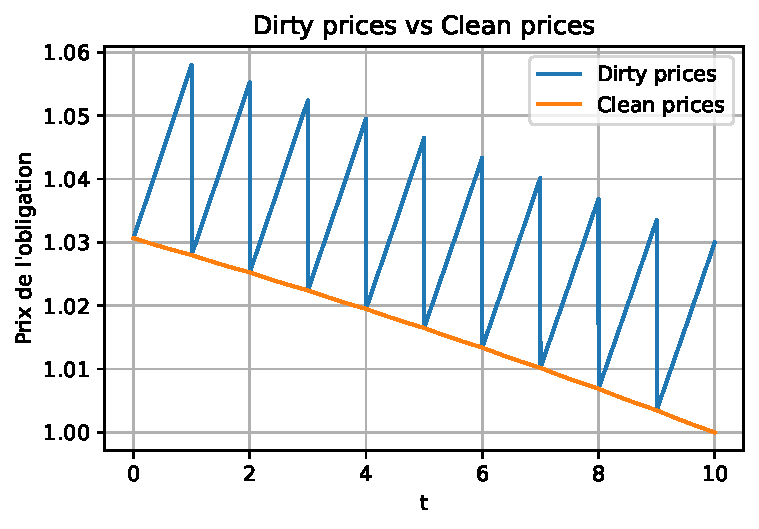
\includegraphics[keepaspectratio]{TP-3_files/figure-pdf/cell-8-output-2.pdf}}

\subsubsection{a. Cas extrêmes}\label{a.-cas-extruxeames}

Nous avons analysé l'évolution du prix de l'obligation dans deux cas
extrêmes afin d'observer l'impact du coupon sur la dynamique des prix.
Toutes choses égales par ailleurs, nous avons modifié le coupon de
l'obligation tout en conservant les autres paramètres constants. Les
deux scénarios étudiés sont les suivants :

\begin{itemize}
\tightlist
\item
  \$ c = 0.01 \$ : le coupon est inférieur au taux d'intérêt sans
  risque.\\
\item
  \$ c = 0.05 \$ : le coupon est supérieur au taux d'intérêt sans
  risque.
\end{itemize}

\paragraph{Cas 1 : \$ c = 0.01 \$}\label{cas-1-c-0.01}

Lorsque \$ c = 1\% \$ et que ce coupon est inférieur au taux d'intérêt
sans risque \$ r \$, la valeur de l'obligation évolue de manière
spécifique :

\begin{itemize}
\tightlist
\item
  Au départ, l'obligation est escomptée car le coupon est faible, et les
  investisseurs anticipent un rendement global inférieur au taux du
  marché.\\
\item
  À mesure que l'échéance approche, l'incertitude sur le paiement du
  coupon disparaît progressivement. Les investisseurs deviennent de plus
  en plus certains que le paiement aura bien lieu.\\
\item
  À la veille du paiement, l'obligation converge vers un prix proche de
  \$ N + c \$ pour le dirty price (car elle inclut le coupon accumulé)
  et \$ N \$ pour le clean price (qui exclut le coupon accumulé).
\end{itemize}

Cela signifie que l'obligation s'apprécie au fil du temps en raison de
la certitude croissante du paiement des flux futurs. En d'autres termes,
plus l'échéance se rapproche, plus l'investisseur est assuré de recevoir
ses paiements, ce qui entraîne une augmentation progressive de la valeur
de l'obligation.

\begin{Shaded}
\begin{Highlighting}[]
\NormalTok{lambda\_ }\OperatorTok{=} \DecValTok{1}\OperatorTok{/}\DecValTok{100}
\NormalTok{r }\OperatorTok{=} \DecValTok{2}\OperatorTok{/}\DecValTok{100}
\NormalTok{T }\OperatorTok{=} \DecValTok{10}
\NormalTok{c1 }\OperatorTok{=} \DecValTok{1}\OperatorTok{/}\DecValTok{100}
\NormalTok{R }\OperatorTok{=} \DecValTok{40}\OperatorTok{/}\DecValTok{100}
\NormalTok{N}\OperatorTok{=}\DecValTok{1}

\NormalTok{clean\_prices1 }\OperatorTok{=}\NormalTok{ []}
\NormalTok{dirty\_prices1 }\OperatorTok{=}\NormalTok{ []}
\ControlFlowTok{for}\NormalTok{ t }\KeywordTok{in}\NormalTok{ grid\_values\_c:}
\NormalTok{    B\_t\_dirty }\OperatorTok{=}\NormalTok{ pricing\_bond(t}\OperatorTok{=}\NormalTok{t,c}\OperatorTok{=}\NormalTok{c1,T}\OperatorTok{=}\NormalTok{T,r}\OperatorTok{=}\NormalTok{r,lambda\_}\OperatorTok{=}\NormalTok{lambda\_,R}\OperatorTok{=}\NormalTok{R,N}\OperatorTok{=}\NormalTok{N)}
\NormalTok{    B\_t\_clean }\OperatorTok{=}\NormalTok{ clean\_price(t}\OperatorTok{=}\NormalTok{t,c}\OperatorTok{=}\NormalTok{c1,T}\OperatorTok{=}\NormalTok{T,r}\OperatorTok{=}\NormalTok{r,lambda\_}\OperatorTok{=}\NormalTok{lambda\_,R}\OperatorTok{=}\NormalTok{R,N}\OperatorTok{=}\NormalTok{N)}
\NormalTok{    clean\_prices1.append(B\_t\_clean)}
\NormalTok{    dirty\_prices1.append(B\_t\_dirty)}

\NormalTok{plt.plot(grid\_values\_c,clean\_prices1, label}\OperatorTok{=}\StringTok{"Clean prices"}\NormalTok{)}
\NormalTok{plt.plot(grid\_values\_c,dirty\_prices1, label}\OperatorTok{=}\StringTok{"Dirty prices"}\NormalTok{)}
\NormalTok{plt.title(}\StringTok{"Clean prices vs Dirty prices"}\NormalTok{)}
\NormalTok{plt.legend()}
\NormalTok{plt.grid()}
\NormalTok{plt.xlabel(}\StringTok{"t"}\NormalTok{)}
\NormalTok{plt.ylabel(}\StringTok{"Prix de l\textquotesingle{}obligation"}\NormalTok{)}
\end{Highlighting}
\end{Shaded}

\begin{verbatim}
Text(0, 0.5, "Prix de l'obligation")
\end{verbatim}

\pandocbounded{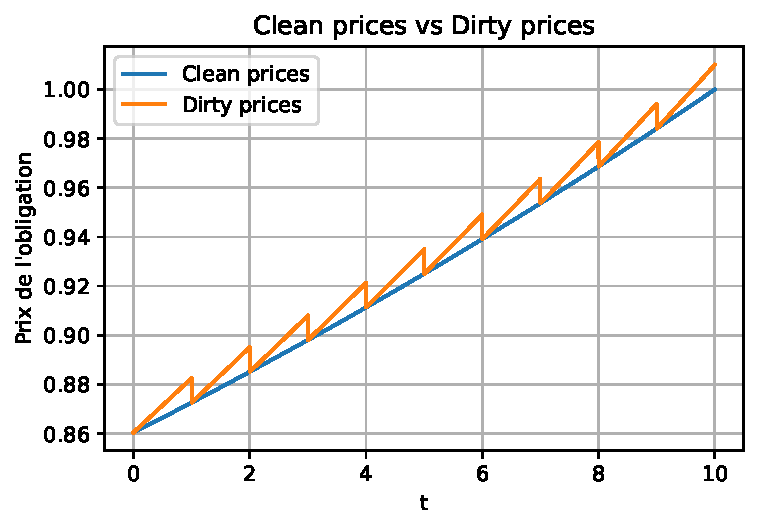
\includegraphics[keepaspectratio]{TP-3_files/figure-pdf/cell-9-output-2.pdf}}

\paragraph{Cas 2 : \$ c = 0.05 \$}\label{cas-2-c-0.05}

Lorsque \$ c = 5\% \$ et que ce coupon est supérieur au taux d'intérêt
sans risque \$ r \$, la dynamique du prix de l'obligation suit une
évolution inverse :

\begin{itemize}
\tightlist
\item
  Au départ, l'obligation est prisée au-dessus du nominal (elle se
  négocie avec une prime). Cela s'explique par le fait que son coupon
  généreux attire les investisseurs, qui considèrent que le rendement
  offert par l'obligation compense largement le risque de crédit et est
  plus attractif que les opportunités de placement à taux sans risque.\\
\item
  À mesure que l'échéance approche, la valeur de l'obligation se
  deprécie progressivement. En effet, à chaque période, l'investisseur
  reçoit un coupon élevé, mais à l'échéance, il ne récupère que le
  nominal \$ N \$, ce qui entraîne une correction progressive du prix de
  marché.\\
\item
  À la veille du remboursement, l'obligation converge vers \$ N + c \$
  pour le dirty price (qui inclut le dernier coupon à verser) et vers \$
  N \$ pour le clean price.
\end{itemize}

Ainsi, cette obligation se déprécie progressivement jusqu'à l'échéance,
car l'effet attractif du coupon élevé s'amenuise à mesure que le
remboursement du capital nominal devient imminent. En d'autres termes,
l'obligation part d'une valeur supérieure à son nominal mais perd
progressivement sa prime à l'approche de l'échéance.

\begin{Shaded}
\begin{Highlighting}[]
\NormalTok{lambda\_ }\OperatorTok{=} \DecValTok{1}\OperatorTok{/}\DecValTok{100}
\NormalTok{r }\OperatorTok{=} \DecValTok{2}\OperatorTok{/}\DecValTok{100}
\NormalTok{T }\OperatorTok{=} \DecValTok{10}
\NormalTok{c2 }\OperatorTok{=} \DecValTok{5}\OperatorTok{/}\DecValTok{100}
\NormalTok{R }\OperatorTok{=} \DecValTok{40}\OperatorTok{/}\DecValTok{100}
\NormalTok{N}\OperatorTok{=}\DecValTok{1}

\NormalTok{clean\_prices2 }\OperatorTok{=}\NormalTok{ []}
\NormalTok{dirty\_prices2 }\OperatorTok{=}\NormalTok{ []}
\ControlFlowTok{for}\NormalTok{ t }\KeywordTok{in}\NormalTok{ grid\_values\_c:}
\NormalTok{    B\_t\_dirty }\OperatorTok{=}\NormalTok{ pricing\_bond(t}\OperatorTok{=}\NormalTok{t,c}\OperatorTok{=}\NormalTok{c2,T}\OperatorTok{=}\NormalTok{T,r}\OperatorTok{=}\NormalTok{r,lambda\_}\OperatorTok{=}\NormalTok{lambda\_,R}\OperatorTok{=}\NormalTok{R,N}\OperatorTok{=}\NormalTok{N)}
\NormalTok{    B\_t\_clean }\OperatorTok{=}\NormalTok{ clean\_price(t}\OperatorTok{=}\NormalTok{t,c}\OperatorTok{=}\NormalTok{c2,T}\OperatorTok{=}\NormalTok{T,r}\OperatorTok{=}\NormalTok{r,lambda\_}\OperatorTok{=}\NormalTok{lambda\_,R}\OperatorTok{=}\NormalTok{R,N}\OperatorTok{=}\NormalTok{N)}
\NormalTok{    clean\_prices2.append(B\_t\_clean)}
\NormalTok{    dirty\_prices2.append(B\_t\_dirty)}

\NormalTok{plt.plot(grid\_values\_c,clean\_prices2, label}\OperatorTok{=}\StringTok{"Clean prices"}\NormalTok{)}
\NormalTok{plt.plot(grid\_values\_c,dirty\_prices2, label}\OperatorTok{=}\StringTok{"Dirty prices"}\NormalTok{)}
\NormalTok{plt.title(}\StringTok{"Clean prices vs Dirty prices"}\NormalTok{)}
\NormalTok{plt.legend()}
\NormalTok{plt.grid()}
\NormalTok{plt.xlabel(}\StringTok{"t"}\NormalTok{)}
\NormalTok{plt.ylabel(}\StringTok{"Prix de l\textquotesingle{}obligation"}\NormalTok{)}
\end{Highlighting}
\end{Shaded}

\begin{verbatim}
Text(0, 0.5, "Prix de l'obligation")
\end{verbatim}

\pandocbounded{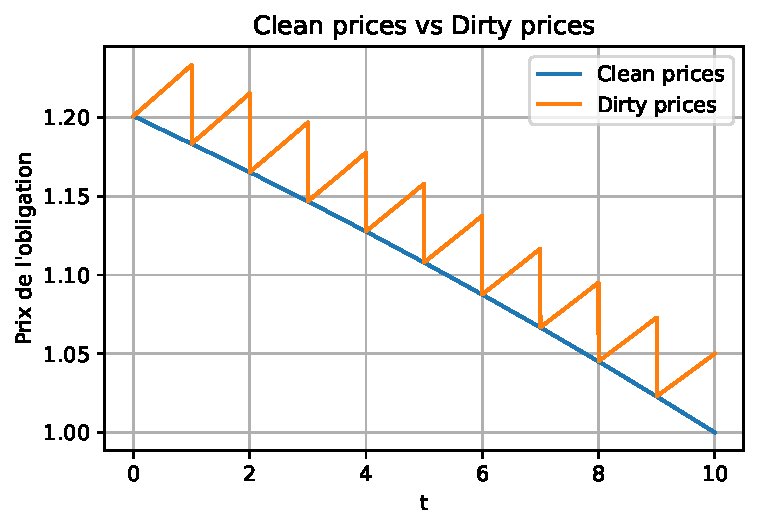
\includegraphics[keepaspectratio]{TP-3_files/figure-pdf/cell-10-output-2.pdf}}

\subsection{III. Évolution du prix en fonction du taux
d'intérêt}\label{iii.-uxe9volution-du-prix-en-fonction-du-taux-dintuxe9ruxeat}

Le prix d'une obligation est une fonction décroissante du taux
d'intérêt. En effet, plus le taux d'intérêt est élevé, plus la valeur
actualisée des flux futurs (coupons et remboursement du nominal) est
faible, ce qui réduit mécaniquement le prix de l'obligation.

Dans cette analyse, il est inutile de distinguer le dirty price et le
clean price, car la différence entre les deux ne dépend pas du taux
d'intérêt. De plus, en considérant \$t = 0
\(, il n'y a pas encore d’intérêts courus (\)c = 0 \$), donc les deux
prix coïncident.

\subsubsection{Obligation au pair}\label{obligation-au-pair}

Autour de \$c - \lambda = 2\% \$, le prix de l'obligation est égal au
nominal. Cela s'explique par le fait que le taux de coupon est
exactement égal au taux de marché. L'obligation est alors dite ``au
pair'', car les investisseurs n'ont ni prime ni décote à appliquer sur
son prix.

\subsubsection{Explication de la relation négative entre prix et
taux}\label{explication-de-la-relation-nuxe9gative-entre-prix-et-taux}

La relation négative entre le prix d'une obligation et le taux d'intérêt
s'explique par l'effet de substitution avec les nouvelles émissions
obligataires.

\begin{itemize}
\tightlist
\item
  Lorsque les taux d'intérêt augmentent, de nouvelles obligations sont
  émises avec des coupons plus attractifs.\\
\item
  En conséquence, les obligations existantes, qui offrent un coupon fixe
  plus faible, deviennent moins intéressantes pour les investisseurs.
  Leur prix diminue afin d'ajuster leur rendement effectif au nouveau
  niveau des taux du marché.\\
\item
  Inversement, si les taux d'intérêt baissent, les obligations
  existantes deviennent plus attractives puisqu'elles offrent un coupon
  plus élevé que les nouvelles émissions, ce qui entraîne une hausse de
  leur prix sur le marché secondaire.
\end{itemize}

Ainsi, la sensibilité d'une obligation aux variations de taux d'intérêt,
appelée ``duration'', est un élément clé dans l'évaluation du risque de
taux et la gestion de portefeuille obligataire.

\begin{Shaded}
\begin{Highlighting}[]
\NormalTok{t}\OperatorTok{=}\DecValTok{0}
\NormalTok{lambda\_ }\OperatorTok{=} \DecValTok{1}\OperatorTok{/}\DecValTok{100}
\NormalTok{T }\OperatorTok{=} \DecValTok{10}
\NormalTok{c }\OperatorTok{=}\DecValTok{3}\OperatorTok{/}\DecValTok{100}
\NormalTok{R }\OperatorTok{=} \DecValTok{40}\OperatorTok{/}\DecValTok{100}
\NormalTok{N}\OperatorTok{=}\DecValTok{1}

\NormalTok{dirty\_prices }\OperatorTok{=}\NormalTok{ []}
\NormalTok{grid\_values\_r }\OperatorTok{=}\NormalTok{ np.arange(}\DecValTok{0}\NormalTok{,}\DecValTok{1}\NormalTok{,}\FloatTok{0.001}\NormalTok{) }
\ControlFlowTok{for}\NormalTok{ r }\KeywordTok{in}\NormalTok{ grid\_values\_r:}
\NormalTok{    B\_t\_dirty }\OperatorTok{=}\NormalTok{ pricing\_bond(t}\OperatorTok{=}\NormalTok{t,c}\OperatorTok{=}\NormalTok{c,T}\OperatorTok{=}\NormalTok{T,r}\OperatorTok{=}\NormalTok{r,lambda\_}\OperatorTok{=}\NormalTok{lambda\_,R}\OperatorTok{=}\NormalTok{R,N}\OperatorTok{=}\NormalTok{N)}
\NormalTok{    dirty\_prices.append(B\_t\_dirty)}

\NormalTok{plt.plot(grid\_values\_r,dirty\_prices, label}\OperatorTok{=}\StringTok{"Dirty prices"}\NormalTok{)}
\NormalTok{plt.title(}\StringTok{"Prix de l\textquotesingle{}obligation en fonction du taux d\textquotesingle{}intérêt"}\NormalTok{)}
\NormalTok{plt.legend()}
\NormalTok{plt.grid()}
\NormalTok{plt.xlabel(}\StringTok{"r"}\NormalTok{)}
\NormalTok{plt.ylabel(}\StringTok{"Prix de l\textquotesingle{}obligation"}\NormalTok{)}
\end{Highlighting}
\end{Shaded}

\begin{verbatim}
Text(0, 0.5, "Prix de l'obligation")
\end{verbatim}

\pandocbounded{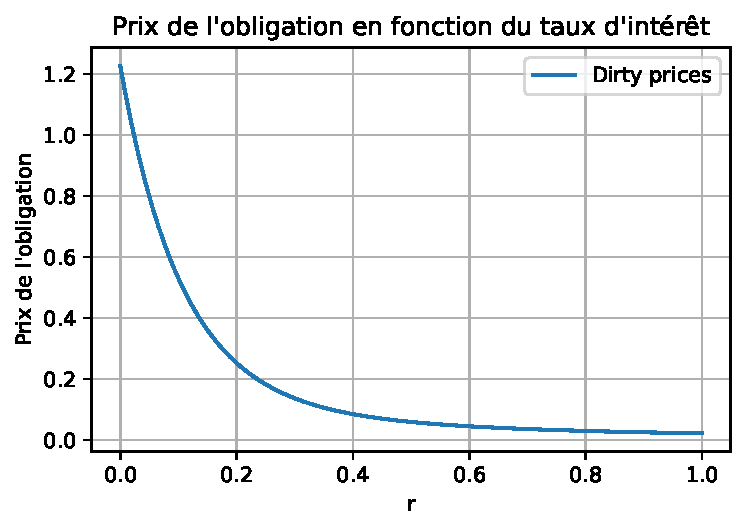
\includegraphics[keepaspectratio]{TP-3_files/figure-pdf/cell-11-output-2.pdf}}

\subsection{IV. Sensibilité du prix de l'obligation au taux d'intérêt /
Duration}\label{iv.-sensibilituxe9-du-prix-de-lobligation-au-taux-dintuxe9ruxeat-duration}

La duration est une mesure de la sensibilité du prix d'une obligation
aux variations du taux d'intérêt. Elle permet d'évaluer le risque de
taux, c'est-à-dire l'impact d'une variation des taux sur la valeur de
l'obligation.

\begin{quote}
Dans le cas de l'évolution du prix en fonction du taux d'intérêt, la
duration sera donc la pente de la courbe représentant cette relation.
\end{quote}

Mathématiquement, la duration est définie comme la dérivée du prix de
l'obligation par rapport au taux d'intérêt :

\[
\delta = - \frac{d B_t}{d r} \times \frac{1}{B_t}
\]

En utilisant une approximation en différences finies, on exprime cette
dérivée de la manière suivante :

\[
\frac{d B_t}{d r}  \approx \frac{B_t(r+\Delta r) - B_t(r)}{\Delta r}
\]

Cette sensibilité permet de mesurer la variation du prix de l'obligation
en réponse à une fluctuation du taux d'intérêt, offrant ainsi une
évaluation directe du risque de taux auquel est exposé l'investisseur.
De ce fait, si les taux d'intérêt bouge de \(\Delta r\) = 1\%, alors les
prix bougeront de -sensibilité * \(\Delta r\) .

Nous allons implémenter ce calcul en Python, en prenant \(\Delta r = 1\)
bp (soit \(0.0001\) en notation décimale).

\begin{Shaded}
\begin{Highlighting}[]
\KeywordTok{def}\NormalTok{ sensivity\_to\_rate(t,c,T,r,lambda\_,R,N,dt}\OperatorTok{=}\DecValTok{1}\NormalTok{,dr}\OperatorTok{=} \FloatTok{0.01}\OperatorTok{/}\DecValTok{100}\NormalTok{):}
    \CommentTok{"""}
\CommentTok{    Fonction qui calcule la sensibilité d\textquotesingle{}une obligation à un taux d\textquotesingle{}intérêt.}
\CommentTok{    """}
\NormalTok{    B\_t }\OperatorTok{=}\NormalTok{ pricing\_bond(t,c,T,r,lambda\_,R,N,dt)}
\NormalTok{    B\_t\_plus }\OperatorTok{=}\NormalTok{ pricing\_bond(t,c,T,r}\OperatorTok{+}\NormalTok{dr,lambda\_,R,N,dt)}
\NormalTok{    sensivity }\OperatorTok{=} \OperatorTok{{-}}\NormalTok{((B\_t\_plus }\OperatorTok{{-}}\NormalTok{ B\_t)}\OperatorTok{/}\NormalTok{dr) }\OperatorTok{*}\NormalTok{ (}\DecValTok{1}\OperatorTok{/}\NormalTok{B\_t)}
    \ControlFlowTok{return}\NormalTok{ sensivity}
\end{Highlighting}
\end{Shaded}

Si les taux d'intérêt bouge de \(\Delta r\) = 1\%, alors les prix
bougeront de -sensibilité * \(\Delta r\) = -8,64 * 1\%. La duration va
être souvent proche de la maturité.

\begin{Shaded}
\begin{Highlighting}[]
\NormalTok{t}\OperatorTok{=}\DecValTok{0}
\NormalTok{lambda\_ }\OperatorTok{=} \DecValTok{1}\OperatorTok{/}\DecValTok{100}
\NormalTok{T }\OperatorTok{=} \DecValTok{10}
\NormalTok{c }\OperatorTok{=}\DecValTok{3}\OperatorTok{/}\DecValTok{100}
\NormalTok{R }\OperatorTok{=} \DecValTok{40}\OperatorTok{/}\DecValTok{100}
\NormalTok{r }\OperatorTok{=} \DecValTok{2}\OperatorTok{/}\DecValTok{100}
\NormalTok{N}\OperatorTok{=}\DecValTok{1}

\NormalTok{sensivity\_to\_rate(t,c,T,r,lambda\_,R,N)}
\end{Highlighting}
\end{Shaded}

\begin{verbatim}
np.float64(8.643982489102903)
\end{verbatim}

D'un point de vue graphique, il existe une certaine identité entre la
maturité et la duration, car cette dernière peut être interprétée comme
le barycentre des flux futurs de l'obligation. Plus ces flux sont
concentrés dans le temps, plus leur pondération affecte la sensibilité
du prix aux variations des taux d'intérêt.

\paragraph{Lien entre duration et
maturité}\label{lien-entre-duration-et-maturituxe9}

\begin{itemize}
\tightlist
\item
  La duration est une approximation de la durée d'exposition au risque,
  ajustée en fonction des flux de paiements.\\
\item
  Elle est souvent proche de la maturité moyenne de l'obligation, bien
  que légèrement inférieure (environ 80\% de la maturité totale, en
  fonction des conditions de marché et du niveau des coupons).
\end{itemize}

Ainsi, plus l'échéance de l'obligation se rapproche, plus la duration
tend à augmenter, car les flux futurs deviennent plus proches dans le
temps, rendant l'obligation plus sensible aux variations des taux
d'intérêt.

\begin{quote}
Lorsque la maturité de l'obligation approche, sa sensibilité au taux
d'intérêt tend à augmenter. En effet, la duration peut être interprétée
comme une mesure du temps moyen pondéré pendant lequel l'investisseur
est exposé au risque de taux.
\end{quote}

\begin{Shaded}
\begin{Highlighting}[]
\NormalTok{t}\OperatorTok{=}\DecValTok{0}
\NormalTok{lambda\_ }\OperatorTok{=} \DecValTok{1}\OperatorTok{/}\DecValTok{100}
\NormalTok{r }\OperatorTok{=} \DecValTok{2}\OperatorTok{/}\DecValTok{100}
\NormalTok{c }\OperatorTok{=}\DecValTok{3}\OperatorTok{/}\DecValTok{100}
\NormalTok{R }\OperatorTok{=} \DecValTok{40}\OperatorTok{/}\DecValTok{100}
\NormalTok{N}\OperatorTok{=}\DecValTok{1}

\NormalTok{dirty\_prices }\OperatorTok{=}\NormalTok{ []}
\NormalTok{grid\_values\_T }\OperatorTok{=}\NormalTok{ np.arange(}\DecValTok{1}\NormalTok{,}\DecValTok{20}\NormalTok{,}\DecValTok{1}\NormalTok{)}
\ControlFlowTok{for}\NormalTok{ T }\KeywordTok{in}\NormalTok{ grid\_values\_T:}
\NormalTok{    B\_t\_dirty }\OperatorTok{=}\NormalTok{ sensivity\_to\_rate(t,c,T,r,lambda\_,R,N)}
\NormalTok{    dirty\_prices.append(B\_t\_dirty)}

\NormalTok{plt.plot(grid\_values\_T,dirty\_prices, label}\OperatorTok{=}\StringTok{"Dirty prices"}\NormalTok{)}
\NormalTok{plt.title(}\StringTok{"Sensibilité en fonction de la maturité"}\NormalTok{)}
\NormalTok{plt.legend()}
\NormalTok{plt.grid()}
\NormalTok{plt.xlabel(}\StringTok{"T"}\NormalTok{)}
\NormalTok{plt.ylabel(}\StringTok{"Sensibilité"}\NormalTok{)}
\end{Highlighting}
\end{Shaded}

\begin{verbatim}
Text(0, 0.5, 'Sensibilité')
\end{verbatim}

\pandocbounded{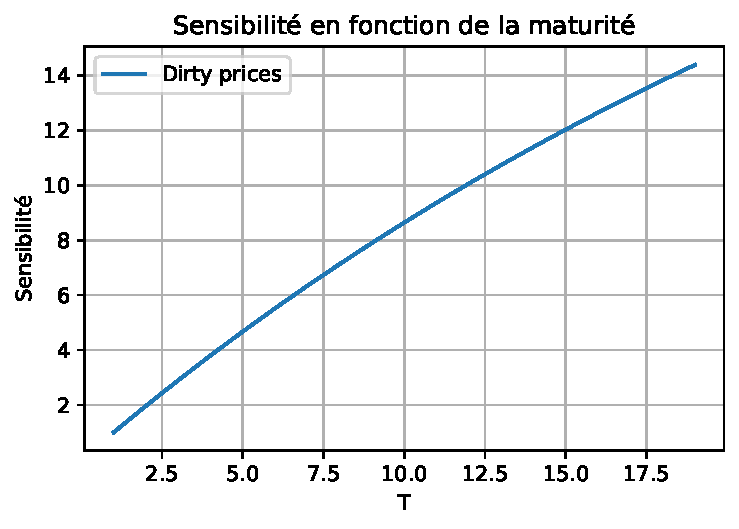
\includegraphics[keepaspectratio]{TP-3_files/figure-pdf/cell-14-output-2.pdf}}

\paragraph{Cas particulier : absence de coupon, de taux d'intérêt et de
risque de
défaut}\label{cas-particulier-absence-de-coupon-de-taux-dintuxe9ruxeat-et-de-risque-de-duxe9faut}

Lorsque le coupon, le taux d'intérêt et l'intensité de défaut sont nuls,
la duration est exactement égale à la maturité de l'obligation. Puisque
la duration peut être interprétée comme le barycentre des flux futurs de
l'obligation, lorsque le coupon et l'intensité de défaut sont nuls, tous
les flux sont concentrés à l'échéance, ce qui équivaut à la maturité de
l'obligation.

\begin{Shaded}
\begin{Highlighting}[]
\NormalTok{t}\OperatorTok{=}\DecValTok{0}
\NormalTok{c }\OperatorTok{=}\NormalTok{ lambda\_ }\OperatorTok{=} \FloatTok{10e{-}6}
\NormalTok{R }\OperatorTok{=} \DecValTok{40}\OperatorTok{/}\DecValTok{100}
\NormalTok{N}\OperatorTok{=}\DecValTok{1}


\NormalTok{dirty\_prices }\OperatorTok{=}\NormalTok{ []}
\ControlFlowTok{for}\NormalTok{ T }\KeywordTok{in}\NormalTok{ grid\_values\_T:}
\NormalTok{    B\_t\_dirty }\OperatorTok{=}\NormalTok{ sensivity\_to\_rate(t,c,T,r,lambda\_,R,N)}
\NormalTok{    dirty\_prices.append(B\_t\_dirty)}

\NormalTok{plt.plot(grid\_values\_T,dirty\_prices, label}\OperatorTok{=}\StringTok{"Dirty prices"}\NormalTok{)}
\NormalTok{plt.title(}\StringTok{"Sensibilité au taux en fonction de la maturité"}\NormalTok{)}
\NormalTok{plt.legend()}
\NormalTok{plt.grid()}
\NormalTok{plt.xlabel(}\StringTok{"T"}\NormalTok{)}
\NormalTok{plt.ylabel(}\StringTok{"Sensibilité"}\NormalTok{)}
\end{Highlighting}
\end{Shaded}

\begin{verbatim}
Text(0, 0.5, 'Sensibilité')
\end{verbatim}

\pandocbounded{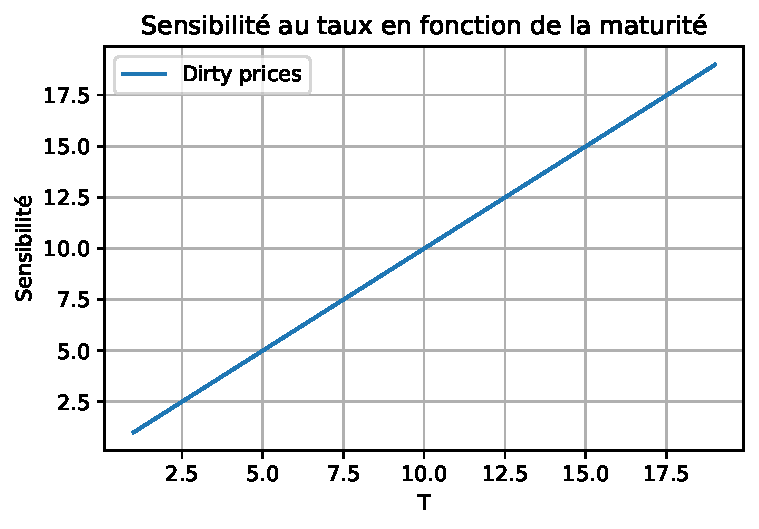
\includegraphics[keepaspectratio]{TP-3_files/figure-pdf/cell-15-output-2.pdf}}

\begin{quote}
Dans le risque de taux, le principale indicateur est la duration.
\end{quote}

\subsection{V. Modèlisation de la
VaR}\label{v.-moduxe8lisation-de-la-var}

\subsubsection{V.1. Approche par la
sensibilité}\label{v.1.-approche-par-la-sensibilituxe9}

Selon le modèle de Hull et White, le taux d'intérêt est modélisé par :

\[
dr = \theta ( \mu - r) dt + \sigma dW
\]

où \(\theta\) est le coefficient de vitesse de réversion, \(\mu\) est le
taux d'intérêt moyen, \(\sigma\) est la volatilité du taux d'intérêt et
\(dW\) est un mouvement brownien. Ce modèle a la spécifité d'être
normale. De ce fait, \(\Delta r \sim N(0, \sigma^2 \Delta t)\). En
faisant l'approximation de la variation du prix, il est possible
d'approcher une VaR par la sensibilité :

\[
\begin{aligned}
Duration &= - \frac{d B_t}{d r} \times \frac{1}{B_t} \\
\frac{d B_t}{B_t} &\approx - Duration \times  \Delta r \\
\end{aligned}
\]

\begin{Shaded}
\begin{Highlighting}[]
\CommentTok{\# Objectif : écrire une fonction qui calcule la VaR avec l\textquotesingle{}approche par duration}
\ImportTok{from}\NormalTok{ scipy.stats }\ImportTok{import}\NormalTok{ norm}

\KeywordTok{def}\NormalTok{ sensitive\_VaR(mu,sigma,t,c,T,r,lambda\_,R,N,h,dt}\OperatorTok{=}\DecValTok{1}\NormalTok{,alpha}\OperatorTok{=}\FloatTok{0.99}\NormalTok{) :}
    \CommentTok{"""}
\CommentTok{    Calcul de la VaR gaussienne}
\CommentTok{    data : les rendements logarithmiques}
\CommentTok{    alpha : le niveau de confiance}
\CommentTok{    """}
\NormalTok{    Duration }\OperatorTok{=}\NormalTok{ sensivity\_to\_rate(t,c,T,r,lambda\_,R,N,dt)}

    \ControlFlowTok{return} \OperatorTok{{-}}\NormalTok{(mu }\OperatorTok{+}\NormalTok{ Duration }\OperatorTok{*}\NormalTok{ sigma }\OperatorTok{*}\NormalTok{ np.sqrt(h) }\OperatorTok{*}\NormalTok{ norm.ppf(}\DecValTok{1} \OperatorTok{{-}}\NormalTok{ alpha))}

\CommentTok{\#{-}{-}{-}{-}{-}{-}{-}{-}{-}{-}{-}{-}{-}{-}{-}{-}{-}{-}{-}{-}{-}{-}{-}{-}{-}{-}{-}{-}{-}{-}{-}{-}{-}{-}{-}{-}{-}{-}}
\CommentTok{\# Paramètres du modèle de taux}
\CommentTok{\#{-}{-}{-}{-}{-}{-}{-}{-}{-}{-}{-}{-}{-}{-}{-}{-}{-}{-}{-}{-}{-}{-}{-}{-}{-}{-}{-}{-}{-}{-}{-}{-}{-}{-}{-}{-}{-}{-}{-}}

\NormalTok{mu }\OperatorTok{=} \DecValTok{0}
\NormalTok{h }\OperatorTok{=} \DecValTok{1}\OperatorTok{/}\DecValTok{12}
\NormalTok{sigma }\OperatorTok{=} \FloatTok{0.01}

\CommentTok{\#{-}{-}{-}{-}{-}{-}{-}{-}{-}{-}{-}{-}{-}{-}{-}{-}{-}{-}{-}{-}{-}{-}{-}{-}{-}{-}{-}{-}{-}{-}{-}{-}{-}{-}{-}{-}{-}{-}}
\CommentTok{\# Paramètres de la valorisation du bond}
\CommentTok{\#{-}{-}{-}{-}{-}{-}{-}{-}{-}{-}{-}{-}{-}{-}{-}{-}{-}{-}{-}{-}{-}{-}{-}{-}{-}{-}{-}{-}{-}{-}{-}{-}{-}{-}{-}{-}{-}{-}{-}}

\NormalTok{t}\OperatorTok{=}\DecValTok{0}
\NormalTok{lambda\_ }\OperatorTok{=} \DecValTok{1}\OperatorTok{/}\DecValTok{100}
\NormalTok{r }\OperatorTok{=} \DecValTok{2}\OperatorTok{/}\DecValTok{100}
\NormalTok{c }\OperatorTok{=}\DecValTok{3}\OperatorTok{/}\DecValTok{100}
\NormalTok{R }\OperatorTok{=} \DecValTok{40}\OperatorTok{/}\DecValTok{100}
\NormalTok{N}\OperatorTok{=}\DecValTok{1}
\NormalTok{T}\OperatorTok{=}\DecValTok{10}

\NormalTok{VaR }\OperatorTok{=}\NormalTok{ sensitive\_VaR(mu,sigma,t,c,T,r,lambda\_,R,N,h}\OperatorTok{=}\NormalTok{h,dt}\OperatorTok{=}\DecValTok{1}\NormalTok{,alpha}\OperatorTok{=}\FloatTok{0.99}\NormalTok{)}
\BuiltInTok{print}\NormalTok{(}\SpecialStringTok{f"VaR estimé par l\textquotesingle{}approche par la sensibilité : }\SpecialCharTok{\{}\NormalTok{VaR}\SpecialCharTok{:.4\%\}}\SpecialStringTok{"}\NormalTok{)}
\end{Highlighting}
\end{Shaded}

\begin{verbatim}
VaR estimé par l'approche par la sensibilité : 5.8049%
\end{verbatim}

Pour cette estimation, nous avions supposé que la volatilité
\(\sigma = 1\%\). Cependant, cette hypothèse pourrait s'écarter de la
réalité. Pour ce faire, nous allons extraire les données de taux
d'intérêt et calculer la volatilité empirique. L'ESTR est un taux un
jour collatéralisé,c'est donc quasiment sans risque. Nous allons donc
utiliser ce taux pour calculer la volatilité empirique. Pour cela, nous
allons utiliser l'historique des taux d'intérêt de l'ESTR sur une
période de 5 ans, i.e.~10/03/2025 - 12/03/2020, disponible sur ce
\href{estr.xlsx}{lien}.

Pour ce faire, nous utilisons la formule suivante :

\[
\sigma = \sqrt{\frac{1}{n-1} \sum_{i=1}^{n} (r_i - \bar{r})^2}
\]

Nous constatons que la volatilité empirique sur les 5 ans est de
25.45\%. Cette valeur est très élevée, ce qui signifie que les taux
d'intérêt ont connu des variations importantes sur cette période. Cela
peut être du à la trop grande période utilisée pour la calibration de la
volatilité. Pour ce faire, nous avons restreint la période à 1 an,
i.e.~10/03/2025 - 10/03/2024. La volatilité empirique sur cette période
est de 1.04\%. Cette valeur est plus cohérente avec les taux d'intérêt
sans risque.

\begin{Shaded}
\begin{Highlighting}[]
\ImportTok{import}\NormalTok{ pandas }\ImportTok{as}\NormalTok{ pd}
\NormalTok{estr\_df }\OperatorTok{=}\NormalTok{ pd.read\_excel(}\StringTok{"estr.xlsx"}\NormalTok{, skiprows}\OperatorTok{=}\DecValTok{6}\NormalTok{)}
\CommentTok{\#date as date}
\NormalTok{estr\_df[}\StringTok{"Date"}\NormalTok{] }\OperatorTok{=}\NormalTok{ pd.to\_datetime(estr\_df[}\StringTok{"Date"}\NormalTok{], }\BuiltInTok{format}\OperatorTok{=}\StringTok{"\%Y{-}\%m{-}}\SpecialCharTok{\%d}\StringTok{"}\NormalTok{)}
\NormalTok{estr\_df }\OperatorTok{=}\NormalTok{ estr\_df.set\_index(}\StringTok{"Date"}\NormalTok{)}
\NormalTok{estr\_df }\OperatorTok{=}\NormalTok{ estr\_df.sort\_index()}

\NormalTok{estr\_df.head()}
\end{Highlighting}
\end{Shaded}

\begin{longtable}[]{@{}lll@{}}
\toprule\noalign{}
& PX\_LAST & CHG\_PCT\_1D \\
Date & & \\
\midrule\noalign{}
\endhead
\bottomrule\noalign{}
\endlastfoot
2020-03-12 & -0.540 & 0.5525 \\
2020-03-13 & -0.541 & -0.1852 \\
2020-03-16 & -0.536 & 0.9242 \\
2020-03-17 & -0.531 & 0.9328 \\
2020-03-18 & -0.529 & 0.3766 \\
\end{longtable}

\begin{Shaded}
\begin{Highlighting}[]
\NormalTok{vol\_est }\OperatorTok{=}\NormalTok{ np.std(estr\_df[}\StringTok{"PX\_LAST"}\NormalTok{].pct\_change())}
\BuiltInTok{print}\NormalTok{(}\SpecialStringTok{f"Volatilité estimée sur 5 ans: }\SpecialCharTok{\{}\NormalTok{vol\_est}\SpecialCharTok{:.4f\}}\SpecialStringTok{"}\NormalTok{)}

\CommentTok{\# volatilité sur 1 an}
\NormalTok{vol\_est}\OperatorTok{=}\NormalTok{ np.std(estr\_df.loc[}\StringTok{"2024{-}03{-}10"}\NormalTok{:}\StringTok{"2025{-}03{-}10"}\NormalTok{, }\StringTok{"PX\_LAST"}\NormalTok{].pct\_change())}
\BuiltInTok{print}\NormalTok{(}\SpecialStringTok{f"Volatilité estimée sur 1 an : }\SpecialCharTok{\{}\NormalTok{vol\_est}\SpecialCharTok{:.4f\}}\SpecialStringTok{"}\NormalTok{)}
\end{Highlighting}
\end{Shaded}

\begin{verbatim}
Volatilité estimée sur 5 ans: 0.2545
Volatilité estimée sur 1 an : 0.0104
\end{verbatim}

\subsubsection{V.2. Approche avec un
repricing}\label{v.2.-approche-avec-un-repricing}

Cette approche consiste à revaloriser, sous l'hypothèse de normalité des
taux, l'obligation à l'instant \(t\) pour un taux \(r + \Delta r\) et de
calculer la perte maximale possible. De ce fait, elle est plus précise
que l'approche par la sensibilité.

Puisque dans le cas d'une obligation, ce dont on veut se prémunir c'est
de la hausse des taux (puisqu'elle fait baisser le taux d'intérêt). De
ce fait, la VaR est donnée par :

\[
\text{VaR} =  - \frac{B_t(r + \Delta r) - B_t }{B_t},
\]

où \(\Delta r\) est la variation des taux d'intérêt.

Par définition, la VaR estimée sera plus basse que l'autre approche en
raison de la convexité de l'évolution du prix de l'obligation en
fonction des taux d'intérêt. La Var par l'approche de la sensibilité,
quant à elle, suppose une linéarité de l'évolution du prix de
l'obligation en fonction des taux d'intérêt.

\begin{Shaded}
\begin{Highlighting}[]
\KeywordTok{def}\NormalTok{ repricing\_VaR(mu,sigma,t,c,T,r,lambda\_,R,N,h,dt}\OperatorTok{=}\DecValTok{1}\NormalTok{,alpha}\OperatorTok{=}\FloatTok{0.99}\NormalTok{) :}
    \CommentTok{"""}
\CommentTok{    Calcul de la VaR gaussienne}
\CommentTok{    data : les rendements logarithmiques}
\CommentTok{    alpha : le niveau de confiance}
\CommentTok{    """}
\NormalTok{    delta\_r }\OperatorTok{=}\NormalTok{ mu }\OperatorTok{+}\NormalTok{ sigma }\OperatorTok{*}\NormalTok{ np.sqrt(h) }\OperatorTok{*}\NormalTok{ norm.ppf(alpha)}
\NormalTok{    P\_t }\OperatorTok{=}\NormalTok{ pricing\_bond(t,c,T,r,lambda\_,R,N,dt)}
\NormalTok{    P\_t\_shocked }\OperatorTok{=}\NormalTok{ pricing\_bond(t,c,T,r}\OperatorTok{+}\NormalTok{delta\_r,lambda\_,R,N,dt)}

\NormalTok{    VAR }\OperatorTok{=} \OperatorTok{{-}}\NormalTok{( (P\_t\_shocked }\OperatorTok{{-}}\NormalTok{ P\_t)}\OperatorTok{/}\NormalTok{P\_t)}

    \ControlFlowTok{return}\NormalTok{ VAR, delta\_r}


\CommentTok{\#{-}{-}{-}{-}{-}{-}{-}{-}{-}{-}{-}{-}{-}{-}{-}{-}{-}{-}{-}{-}{-}{-}{-}{-}{-}{-}{-}{-}{-}{-}{-}{-}{-}{-}{-}{-}{-}{-}}
\CommentTok{\# Paramètres du modèle de taux}
\CommentTok{\#{-}{-}{-}{-}{-}{-}{-}{-}{-}{-}{-}{-}{-}{-}{-}{-}{-}{-}{-}{-}{-}{-}{-}{-}{-}{-}{-}{-}{-}{-}{-}{-}{-}{-}{-}{-}{-}{-}{-}}
\NormalTok{mu }\OperatorTok{=} \DecValTok{0}
\NormalTok{h }\OperatorTok{=} \DecValTok{1}\OperatorTok{/}\DecValTok{12}
\NormalTok{sigma }\OperatorTok{=} \FloatTok{0.01}

\CommentTok{\#{-}{-}{-}{-}{-}{-}{-}{-}{-}{-}{-}{-}{-}{-}{-}{-}{-}{-}{-}{-}{-}{-}{-}{-}{-}{-}{-}{-}{-}{-}{-}{-}{-}{-}{-}{-}{-}{-}}
\CommentTok{\# Paramètres de la valorisation du bond}
\CommentTok{\#{-}{-}{-}{-}{-}{-}{-}{-}{-}{-}{-}{-}{-}{-}{-}{-}{-}{-}{-}{-}{-}{-}{-}{-}{-}{-}{-}{-}{-}{-}{-}{-}{-}{-}{-}{-}{-}{-}{-}}
\NormalTok{t}\OperatorTok{=}\DecValTok{0}
\NormalTok{lambda\_ }\OperatorTok{=} \DecValTok{1}\OperatorTok{/}\DecValTok{100}
\NormalTok{r }\OperatorTok{=} \DecValTok{2}\OperatorTok{/}\DecValTok{100}
\NormalTok{c }\OperatorTok{=}\DecValTok{3}\OperatorTok{/}\DecValTok{100}
\NormalTok{R }\OperatorTok{=} \DecValTok{40}\OperatorTok{/}\DecValTok{100}
\NormalTok{N}\OperatorTok{=}\DecValTok{1}
\NormalTok{T}\OperatorTok{=}\DecValTok{10}

\NormalTok{VaR, delta\_r }\OperatorTok{=}\NormalTok{ repricing\_VaR(mu,sigma,t,c,T,r,lambda\_,R,N,h}\OperatorTok{=}\NormalTok{h,dt}\OperatorTok{=}\DecValTok{1}\NormalTok{,alpha}\OperatorTok{=}\FloatTok{0.99}\NormalTok{)}

\BuiltInTok{print}\NormalTok{(}\SpecialStringTok{f"VaR estimé par l\textquotesingle{}approche par le réajustement : }\SpecialCharTok{\{}\NormalTok{VaR}\SpecialCharTok{:.4\%\}}\SpecialStringTok{"}\NormalTok{)}
\BuiltInTok{print}\NormalTok{(}\SpecialStringTok{f"Choc de taux : }\SpecialCharTok{\{}\NormalTok{delta\_r}\SpecialCharTok{:.2\%\}}\SpecialStringTok{"}\NormalTok{)}
\end{Highlighting}
\end{Shaded}

\begin{verbatim}
VaR estimé par l'approche par le réajustement : 5.6272%
Choc de taux : 0.67%
\end{verbatim}

\subsection{VI. Focus risque de crédit \&
contrepartie}\label{vi.-focus-risque-de-cruxe9dit-contrepartie}

Le risque de crédit est le risque que l'émetteur d'une obligation ne
soit pas en mesure de respecter ses engagements financiers, entraînant
ainsi des pertes pour les investisseurs. Ce risque est particulièrement
pertinent dans le contexte des obligations, car il peut affecter la
valeur de l'obligation et la capacité de l'investisseur à récupérer son
capital. Le risque de contrepartie, quant à lui, est le risque que la
contrepartie d'une transaction financière ne respecte pas ses
obligations contractuelles. Dans le cas des obligations, cela peut se
traduire par le non-paiement des coupons ou du capital à l'échéance. Ce
risque est particulièrement important dans les transactions de gré à gré
(OTC), où les parties ne sont pas soumises aux mêmes exigences
réglementaires que celles des marchés organisés.

\subsubsection{VI.1. Comment estimer l'intensité de défaut
?}\label{vi.1.-comment-estimer-lintensituxe9-de-duxe9faut}

Précedemment, nous avons valoriser l'obligation de la manière suivante :

\[
\begin{aligned}
B_t &= C_t + N_t + R_t \\
&= N \left[ \sum_{i=1}^{n}  c \times e^{-(r + \lambda) \times (T_i
-t)} \mathbb{1}_{T_i \geq t} + e^{-(r+\lambda)(T-t)} \mathbb{1}_{T \geq t} +  \lambda R \times \frac{1 - e^{-(r+\lambda)(T-t)}}{r+\lambda} \mathbb{1}_{T \geq t} \right]
\end{aligned}
\]

et nous avons signfié la condition dans laquelle l'obligation émise vaut
100\% du nominal, i.e.~au pair, est \(c \approx r + \lambda\).
Cependant, ce n'est pas exact.

Soit un coupon payé en continu, la valorisation de l'obligation est
donnée par :

\[
\begin{aligned}
B_t &= N \left[ \int_{t}^{T} c e^{-(r + \lambda) \times (u-t)} du + e^{-(r+\lambda)(T-t)} +  \lambda R \times \frac{1 - e^{-(r+\lambda)(T-t)}}{r+\lambda} \right]\\
&= N \left[ \frac{c}{r + \lambda} \left(1 - e^{-(r + \lambda)(T-t)} \right) + e^{-(r+\lambda)(T-t)} +  \lambda R \times \frac{1 - e^{-(r+\lambda)(T-t)}}{r+\lambda} \right]\\
B_t = N &\Leftrightarrow c = r + \lambda (1 - R) \\
& c - r = \lambda (1 - R) 
\end{aligned}
\]

De ce fait, en extrayant \(c\), la condition dans laquelle l'obligation
émise vaut 100\% du nominal, i.e.~au pair, est \$c = r + \lambda (1 - R)
\$.

\begin{quote}
💡 \(s = c-r\) est la prime de crédit ou encore le spread de crédit.
C'est la prime que l'investisseur demande pour le risque de crédit. Si
\(c > r\), l'obligation est émise à un prix supérieur à 100\% du
nominal. Si \(c < r\), l'obligation est émise à un prix inférieur à
100\% du nominal. Ce spread permet de faire la relation entre la PD
exprimé par \(\lambda\) et la LGD exprimé par \(1 -R\). Cette
information est plus facile à avoir que l'intensité de défaut car le
spread est coté sur le marché à travers les CDS. Par définition, on en
déduit facilement que plus cettre prime est élevé, plus l'emetteur est
risqué.
\end{quote}

\begin{quote}
Take away : Les notions de duration et de spread sont très importants
dans la modélisation du risque de taux
\end{quote}

\paragraph{cas de l'argentine, pays
risqué}\label{cas-de-largentine-pays-risquuxe9}

\begin{Shaded}
\begin{Highlighting}[]
\NormalTok{s }\OperatorTok{=} \DecValTok{1031}\OperatorTok{/}\DecValTok{10000} 
\NormalTok{R }\OperatorTok{=} \FloatTok{0.4}
\NormalTok{lambda\_ }\OperatorTok{=}\NormalTok{ s }\OperatorTok{/}\NormalTok{ (}\DecValTok{1} \OperatorTok{{-}}\NormalTok{ R)}
\NormalTok{t}\OperatorTok{=}\DecValTok{0}

\BuiltInTok{print}\NormalTok{(}\SpecialStringTok{f"Spread de crédit : }\SpecialCharTok{\{}\NormalTok{s}\SpecialCharTok{:.2\%\}}\SpecialStringTok{"}\NormalTok{)}
\BuiltInTok{print}\NormalTok{(}\SpecialStringTok{f"Recouvrement : }\SpecialCharTok{\{}\NormalTok{R}\SpecialCharTok{:.2\%\}}\SpecialStringTok{"}\NormalTok{)}
\BuiltInTok{print}\NormalTok{(}\SpecialStringTok{f"Intensité de défaut : }\SpecialCharTok{\{}\NormalTok{lambda\_}\SpecialCharTok{:.2\%\}}\SpecialStringTok{"}\NormalTok{)}
\NormalTok{PS }\OperatorTok{=}\NormalTok{ [np.exp( }\OperatorTok{{-}}\NormalTok{ lambda\_ }\OperatorTok{*}\NormalTok{ (T }\OperatorTok{{-}}\NormalTok{ t)) }\ControlFlowTok{for}\NormalTok{ T }\KeywordTok{in} \BuiltInTok{range}\NormalTok{(}\DecValTok{1}\NormalTok{, }\DecValTok{21}\NormalTok{)]}

\NormalTok{plt.plot(}\BuiltInTok{range}\NormalTok{(}\DecValTok{1}\NormalTok{,}\DecValTok{21}\NormalTok{),PS)}
\NormalTok{plt.title(}\StringTok{"Probabilité de survie en fonction de la maturité"}\NormalTok{)}
\NormalTok{plt.xlabel(}\StringTok{"T"}\NormalTok{)}
\NormalTok{plt.ylabel(}\StringTok{"Probabilité de survie"}\NormalTok{)}
\NormalTok{plt.grid()}
\end{Highlighting}
\end{Shaded}

\begin{verbatim}
Spread de crédit : 10.31%
Recouvrement : 40.00%
Intensité de défaut : 17.18%
\end{verbatim}

\pandocbounded{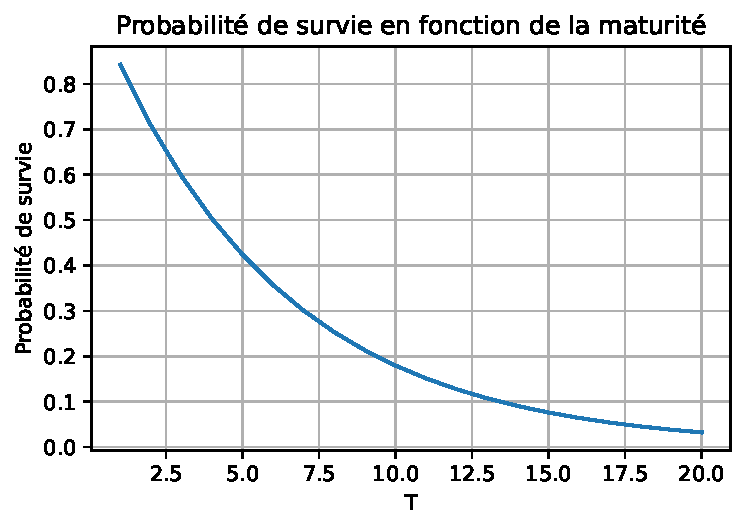
\includegraphics[keepaspectratio]{TP-3_files/figure-pdf/cell-20-output-2.pdf}}

\paragraph{cas de la France}\label{cas-de-la-france}

\begin{Shaded}
\begin{Highlighting}[]
\CommentTok{\# Cas de la France}
\NormalTok{s }\OperatorTok{=} \FloatTok{32.4}\OperatorTok{/}\DecValTok{10000} 
\NormalTok{R }\OperatorTok{=} \FloatTok{0.4}
\NormalTok{lambda\_ }\OperatorTok{=}\NormalTok{ s }\OperatorTok{/}\NormalTok{ (}\DecValTok{1} \OperatorTok{{-}}\NormalTok{ R)}
\NormalTok{t}\OperatorTok{=}\DecValTok{0}

\BuiltInTok{print}\NormalTok{(}\SpecialStringTok{f"Spread de crédit : }\SpecialCharTok{\{}\NormalTok{s}\SpecialCharTok{:.2\%\}}\SpecialStringTok{"}\NormalTok{)}
\BuiltInTok{print}\NormalTok{(}\SpecialStringTok{f"Recouvrement : }\SpecialCharTok{\{}\NormalTok{R}\SpecialCharTok{:.2\%\}}\SpecialStringTok{"}\NormalTok{)}
\BuiltInTok{print}\NormalTok{(}\SpecialStringTok{f"Intensité de défaut : }\SpecialCharTok{\{}\NormalTok{lambda\_}\SpecialCharTok{:.2\%\}}\SpecialStringTok{"}\NormalTok{)}
\NormalTok{PS }\OperatorTok{=}\NormalTok{ [np.exp( }\OperatorTok{{-}}\NormalTok{ lambda\_ }\OperatorTok{*}\NormalTok{ (T }\OperatorTok{{-}}\NormalTok{ t)) }\ControlFlowTok{for}\NormalTok{ T }\KeywordTok{in} \BuiltInTok{range}\NormalTok{(}\DecValTok{1}\NormalTok{, }\DecValTok{21}\NormalTok{)]}

\NormalTok{plt.plot(}\BuiltInTok{range}\NormalTok{(}\DecValTok{1}\NormalTok{,}\DecValTok{21}\NormalTok{),PS)}
\NormalTok{plt.title(}\StringTok{"Probabilité de survie en fonction de la maturité"}\NormalTok{)}
\NormalTok{plt.xlabel(}\StringTok{"T"}\NormalTok{)}
\NormalTok{plt.ylabel(}\StringTok{"Probabilité de survie"}\NormalTok{)}
\NormalTok{plt.grid()}
\end{Highlighting}
\end{Shaded}

\begin{verbatim}
Spread de crédit : 0.32%
Recouvrement : 40.00%
Intensité de défaut : 0.54%
\end{verbatim}

\pandocbounded{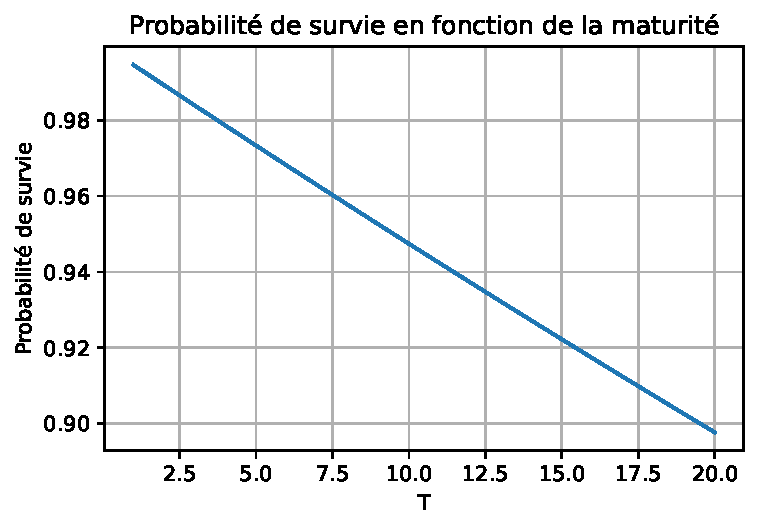
\includegraphics[keepaspectratio]{TP-3_files/figure-pdf/cell-21-output-2.pdf}}

En comparant les deux pays, l'Argentine et la France. On sait que
l'argentine est un pays plus risqué que la France. Cela se voit
également au niveau des spreads de crédit. En effet, le spread de
l'Argentine est plus élevé que celui de la France. Cela signifie que les
investisseurs demandent une prime de risque plus élevée pour investir
dans des obligations argentines que dans des obligations françaises. De
plus, en regardant la probabilité de survie des deux pays, on constate
que la probabilité de survie de l'Argentine est plus faible que celle de
la France. Cela signifie que les investisseurs considèrent que
l'Argentine est plus susceptible de faire défaut que la France.

\subsubsection{VI.2 Sensibilité
crédit}\label{vi.2-sensibilituxe9-cruxe9dit}

\begin{Shaded}
\begin{Highlighting}[]
\KeywordTok{def}\NormalTok{ sensivity\_to\_credit(t,c,T,r,lambda\_,R,N,dt}\OperatorTok{=}\DecValTok{1}\NormalTok{,dlambda\_}\OperatorTok{=} \FloatTok{0.01}\OperatorTok{/}\DecValTok{100}\NormalTok{):}
    \CommentTok{"""}
\CommentTok{    Fonction qui calcule la sensibilité d\textquotesingle{}une obligation à un taux d\textquotesingle{}intérêt.}
\CommentTok{    """}
\NormalTok{    B\_t }\OperatorTok{=}\NormalTok{ pricing\_bond(t,c,T,r,lambda\_,R,N,dt)}
\NormalTok{    B\_t\_plus }\OperatorTok{=}\NormalTok{ pricing\_bond(t,c,T,r,lambda\_ }\OperatorTok{+}\NormalTok{ dlambda\_,R,N,dt)}
    
\NormalTok{    sensivity }\OperatorTok{=} \OperatorTok{{-}}\NormalTok{((B\_t\_plus }\OperatorTok{{-}}\NormalTok{ B\_t)}\OperatorTok{/}\NormalTok{dlambda\_) }\OperatorTok{*}\NormalTok{ (}\DecValTok{1}\OperatorTok{/}\NormalTok{B\_t) }\OperatorTok{*}\NormalTok{ (}\DecValTok{1}\OperatorTok{/}\NormalTok{ (}\DecValTok{1}\OperatorTok{{-}}\NormalTok{R))}

    \ControlFlowTok{return}\NormalTok{ sensivity}
\end{Highlighting}
\end{Shaded}

\begin{Shaded}
\begin{Highlighting}[]
\NormalTok{t}\OperatorTok{=}\DecValTok{0}
\NormalTok{lambda\_ }\OperatorTok{=} \DecValTok{1}\OperatorTok{/}\DecValTok{100}
\NormalTok{T }\OperatorTok{=} \DecValTok{10}
\NormalTok{c }\OperatorTok{=}\DecValTok{3}\OperatorTok{/}\DecValTok{100}
\NormalTok{R }\OperatorTok{=} \DecValTok{40}\OperatorTok{/}\DecValTok{100}
\NormalTok{r }\OperatorTok{=} \DecValTok{2}\OperatorTok{/}\DecValTok{100}
\NormalTok{N}\OperatorTok{=}\DecValTok{1}

\NormalTok{sensivity\_to\_credit(t,c,T,r,lambda\_,R,N,dlambda\_}\OperatorTok{=}\FloatTok{0.01}\OperatorTok{/}\DecValTok{100}\NormalTok{)}
\end{Highlighting}
\end{Shaded}

\begin{verbatim}
np.float64(8.821190868023761)
\end{verbatim}

\begin{Shaded}
\begin{Highlighting}[]
\NormalTok{t}\OperatorTok{=}\DecValTok{0}
\NormalTok{lambda\_ }\OperatorTok{=} \DecValTok{1}\OperatorTok{/}\DecValTok{100}
\NormalTok{r }\OperatorTok{=} \DecValTok{2}\OperatorTok{/}\DecValTok{100}
\NormalTok{c }\OperatorTok{=}\DecValTok{3}\OperatorTok{/}\DecValTok{100}
\NormalTok{R }\OperatorTok{=} \DecValTok{40}\OperatorTok{/}\DecValTok{100}
\NormalTok{N}\OperatorTok{=}\DecValTok{1}

\NormalTok{dirty\_prices }\OperatorTok{=}\NormalTok{ []}
\NormalTok{grid\_values\_T }\OperatorTok{=}\NormalTok{ np.arange(}\DecValTok{1}\NormalTok{,}\DecValTok{20}\NormalTok{,}\DecValTok{1}\NormalTok{)}
\ControlFlowTok{for}\NormalTok{ T }\KeywordTok{in}\NormalTok{ grid\_values\_T:}
\NormalTok{    B\_t\_dirty }\OperatorTok{=}\NormalTok{ sensivity\_to\_credit(t,c,T,r,lambda\_,R,N)}
\NormalTok{    dirty\_prices.append(B\_t\_dirty)}

\NormalTok{plt.plot(grid\_values\_T,dirty\_prices, label}\OperatorTok{=}\StringTok{"Dirty prices"}\NormalTok{)}
\NormalTok{plt.title(}\StringTok{"Sensibilité crédit en fonction de la maturité"}\NormalTok{)}
\NormalTok{plt.legend()}
\NormalTok{plt.grid()}
\NormalTok{plt.xlabel(}\StringTok{"T"}\NormalTok{)}
\NormalTok{plt.ylabel(}\StringTok{"Sensibilité"}\NormalTok{)}
\end{Highlighting}
\end{Shaded}

\begin{verbatim}
Text(0, 0.5, 'Sensibilité')
\end{verbatim}

\pandocbounded{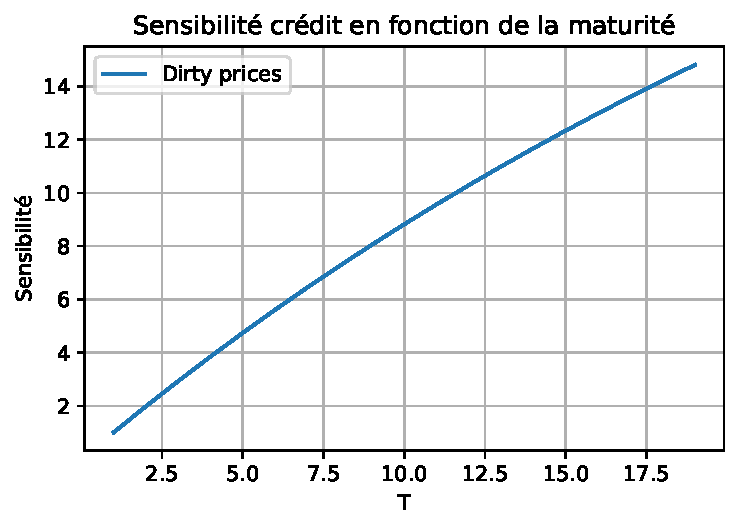
\includegraphics[keepaspectratio]{TP-3_files/figure-pdf/cell-24-output-2.pdf}}

Soit le modèle normale pour le taux :

\[
dr_t = \theta (\mu - r_t) dt + \sigma_r dW_t
\]

et un modèle log normale pour le spread de crédit, puisqu'il ne peut
être négatif : \[
\frac{ds_t}{s_t} = \sigma_s dZ_t
\]

Ces deux modèles sont liés par \(dW_t dZ_t = \rho dt\). On peut exprimer
cette relation par \(Z_t = \rho W_t + \sqrt{1 - \rho^2} V_t\), où
\(V_t\) est un mouvement brownien standard indépendant de \(W_t\). Cette
corrélation est positive. \textgreater{} 💡 si les taux d'intérêt
montent, le risque de crédit augmente puisque les entreprises ont plus
de mal à rembourser leur dette. De ce fait, le spread de crédit
augmente.

Supposons qu'on cherche à calculer une VaR d'horizon \(h\). Pour cela,
il faudra faire des simulations de Monte Carlo pour les deux modèles.

\[
\begin{aligned}
r_{t+h} &= r_t + \theta (\mu - r_t) h + \sigma_r \sqrt{h} W_t \\
s_{t+h} &= s_t \exp(\sigma_s \sqrt{h} Z_t) \\
ou \quad s_{t+h} &= s_t (1 + \sigma_s \sqrt{h} Z_t) \quad (\text{par DL})
\end{aligned}
\]

Posons les paramètres suivants :

\begin{itemize}
\tightlist
\item
  \(\theta = 0.1\) : le coefficient de vitesse de réversion
\item
  \(\mu = 0.02\) : le taux d'intérêt moyen
\item
  \(\sigma_r = 0.01\) : la volatilité du taux d'intérêt
\item
  \(\sigma_s = 0.4\) : la volatilité du spread de crédit
\item
  \(\rho = 0.4\) : la corrélation entre les deux mouvements browniens
\item
  \(r = 0.02\) : le taux d'intérêt initial
\item
  \(h = 1/12\) : l'horizon de calcul de la VaR
\item
  \(c = 3\%\) : le coupon annuel
\item
  \(R = 40\%\) : le taux de recouvrement
\item
  \(N = 1\) : le nominal de l'obligation
\item
  \(T = 10\) : l'échéance de l'obligation
\end{itemize}

\begin{Shaded}
\begin{Highlighting}[]
\ImportTok{import}\NormalTok{ numpy }\ImportTok{as}\NormalTok{ np}

\KeywordTok{def}\NormalTok{ MC\_VaR(c,T,r,lambda\_,R,N,h,sigma\_r, sigma\_s, rho, alpha}\OperatorTok{=}\FloatTok{0.99}\NormalTok{, N\_MC}\OperatorTok{=}\DecValTok{1000}\NormalTok{,dt}\OperatorTok{=}\DecValTok{1}\NormalTok{):}
    \CommentTok{\# print("Parameters")}
    \CommentTok{\# print(f"coupon : \{c:.2\%\}")}
    \CommentTok{\# print(f"maturity : \{T\} years")}
    \CommentTok{\# print(f"risk free rate : \{r:.2\%\}")}
    \CommentTok{\# print(f"credit spread : \{lambda\_:.2\%\}")}
    \CommentTok{\# print(f"recovery rate : \{R:.2\%\}")}
    \CommentTok{\# print(f"nominal : \{N\}")}

\NormalTok{    prices }\OperatorTok{=}\NormalTok{ []}
    
\NormalTok{    P\_0 }\OperatorTok{=}\NormalTok{ pricing\_bond(t}\OperatorTok{=}\DecValTok{0}\NormalTok{,c}\OperatorTok{=}\NormalTok{c,T}\OperatorTok{=}\NormalTok{T,r}\OperatorTok{=}\NormalTok{r,lambda\_}\OperatorTok{=}\NormalTok{lambda\_,R}\OperatorTok{=}\NormalTok{R,N}\OperatorTok{=}\NormalTok{N,dt}\OperatorTok{=}\NormalTok{dt)}
    \CommentTok{\# print(f"P0 : \{P\_0\}")}

\NormalTok{    s\_0 }\OperatorTok{=}\NormalTok{ lambda\_ }\OperatorTok{*}\NormalTok{ (}\DecValTok{1} \OperatorTok{{-}}\NormalTok{ R)}
\NormalTok{    r\_0 }\OperatorTok{=}\NormalTok{ r}

    \ControlFlowTok{for}\NormalTok{ t }\KeywordTok{in} \BuiltInTok{range}\NormalTok{(N\_MC):}
        \CommentTok{\# Generate correlated Brownian motions}
\NormalTok{        W1 }\OperatorTok{=}\NormalTok{ np.random.normal()}
\NormalTok{        W2 }\OperatorTok{=}\NormalTok{ rho }\OperatorTok{*}\NormalTok{ W1 }\OperatorTok{+}\NormalTok{ np.sqrt(}\DecValTok{1} \OperatorTok{{-}}\NormalTok{ rho) }\OperatorTok{*}\NormalTok{ np.random.normal()}

        \CommentTok{\# Euler discretization }
\NormalTok{        r\_h }\OperatorTok{=}\NormalTok{ r\_0 }\OperatorTok{+}\NormalTok{ sigma\_r }\OperatorTok{*}\NormalTok{ np.sqrt(h) }\OperatorTok{*}\NormalTok{ W1}
\NormalTok{        s\_h }\OperatorTok{=}\NormalTok{ s\_0 }\OperatorTok{*}\NormalTok{ ( }\DecValTok{1} \OperatorTok{+}\NormalTok{ sigma\_s }\OperatorTok{*}\NormalTok{ np.sqrt(h) }\OperatorTok{*}\NormalTok{ W2)}
\NormalTok{        lambda\_h }\OperatorTok{=}\NormalTok{ s\_h }\OperatorTok{/}\NormalTok{ (}\DecValTok{1} \OperatorTok{{-}}\NormalTok{ R)}
        \CommentTok{\# print("="*30)}
        \CommentTok{\# print("Parameters")}
        \CommentTok{\# print(f"coupon : \{c:.2\%\}")}
        \CommentTok{\# print(f"maturity : \{T\} years")}
        \CommentTok{\# print(f"risk free rate : \{r\_h:.2\%\}")}
        \CommentTok{\# print(f"credit spread : \{lambda\_h:.2\%\}")}
        \CommentTok{\# print(f"recovery rate : \{R:.2\%\}")}
        \CommentTok{\# print(f"nominal : \{N\}")}

\NormalTok{        P\_h }\OperatorTok{=}\NormalTok{ pricing\_bond(t}\OperatorTok{=}\NormalTok{h,c}\OperatorTok{=}\NormalTok{c,T}\OperatorTok{=}\NormalTok{T,r}\OperatorTok{=}\NormalTok{r\_h,lambda\_ }\OperatorTok{=}\NormalTok{ lambda\_h,R}\OperatorTok{=}\NormalTok{R,N}\OperatorTok{=}\NormalTok{N,dt}\OperatorTok{=}\NormalTok{dt)}
        \CommentTok{\# print(f"Price : \{P\_h\}")}
\NormalTok{        variation }\OperatorTok{=}\NormalTok{ (P\_h }\OperatorTok{{-}}\NormalTok{ P\_0)}\OperatorTok{/}\NormalTok{P\_0}
\NormalTok{        prices.append(variation)}


\NormalTok{    VaR }\OperatorTok{=}\NormalTok{ np.quantile(prices, }\DecValTok{1} \OperatorTok{{-}}\NormalTok{ alpha)}

    \ControlFlowTok{return}\NormalTok{ VaR}

\NormalTok{sigma\_r }\OperatorTok{=} \FloatTok{0.01}
\NormalTok{sigma\_s }\OperatorTok{=} \FloatTok{0.4}
\NormalTok{rho }\OperatorTok{=} \FloatTok{0.40}

\NormalTok{lambda\_ }\OperatorTok{=} \DecValTok{1}\OperatorTok{/}\DecValTok{100}
\NormalTok{r }\OperatorTok{=} \DecValTok{2}\OperatorTok{/}\DecValTok{100}
\NormalTok{c }\OperatorTok{=}\DecValTok{3}\OperatorTok{/}\DecValTok{100}
\NormalTok{R }\OperatorTok{=} \DecValTok{40}\OperatorTok{/}\DecValTok{100}
\NormalTok{N}\OperatorTok{=}\DecValTok{1}
\NormalTok{h }\OperatorTok{=} \DecValTok{1}\OperatorTok{/}\DecValTok{12}
\NormalTok{T}\OperatorTok{=} \DecValTok{10}

\NormalTok{VaR\_monte\_carlo }\OperatorTok{=}\NormalTok{ MC\_VaR(c,T,r,lambda\_,R,N,h,sigma\_r, sigma\_s, rho, alpha}\OperatorTok{=}\FloatTok{0.99}\NormalTok{, N\_MC}\OperatorTok{=}\DecValTok{1000}\NormalTok{,dt}\OperatorTok{=}\DecValTok{1}\NormalTok{)}
\BuiltInTok{print}\NormalTok{(}\SpecialStringTok{f"VaR estimé par Monte Carlo : }\SpecialCharTok{\{}\NormalTok{VaR\_monte\_carlo}\SpecialCharTok{:.4\%\}}\SpecialStringTok{"}\NormalTok{)}
\end{Highlighting}
\end{Shaded}

\begin{verbatim}
VaR estimé par Monte Carlo : -5.7604%
\end{verbatim}

Lorsque \$ \rho \$ (le coefficient de corrélation entre les taux
d'intérêt et le spread de crédit) est positif, une hausse des taux
d'intérêt entraîne également une hausse du spread de crédit. Cette
dynamique amplifie le risque global, car les pertes dues à la hausse des
taux s'ajoutent aux pertes induites par l'élargissement du spread de
crédit. Ainsi, la Value at Risk (VaR) est plus élevée, reflétant
l'accumulation des risques liés aux deux facteurs.

En revanche, lorsque \$ \rho \$ est négatif, une hausse des taux
d'intérêt tend à réduire le spread de crédit, et inversement. Il se crée
alors un effet de compensation : les pertes générées par l'évolution des
taux sont partiellement absorbées par les gains résultant de la
contraction du spread (ou inversement). C'est le principe de
diversification. Dans ce cas, la VaR est plus faible, car les effets du
taux d'intérêt et du spread de crédit s'annulent en partie, réduisant
ainsi l'ampleur des pertes potentielles.

\begin{Shaded}
\begin{Highlighting}[]
\CommentTok{\# VaR en fonction de rho}
\ImportTok{from}\NormalTok{ tqdm }\ImportTok{import}\NormalTok{ tqdm }

\NormalTok{rhos }\OperatorTok{=}\NormalTok{ np.linspace(}\OperatorTok{{-}}\DecValTok{1}\NormalTok{,}\DecValTok{1}\NormalTok{,}\DecValTok{100}\NormalTok{)}
\NormalTok{VaRs }\OperatorTok{=}\NormalTok{ [MC\_VaR(c,T,r,lambda\_,R,N,h,sigma\_r, sigma\_s, rho, alpha}\OperatorTok{=}\FloatTok{0.99}\NormalTok{, N\_MC}\OperatorTok{=}\DecValTok{1000}\NormalTok{,dt}\OperatorTok{=}\DecValTok{1}\NormalTok{) }\ControlFlowTok{for}\NormalTok{ rho }\KeywordTok{in}\NormalTok{ tqdm(rhos)]}

\NormalTok{plt.plot(rhos,VaRs)}
\NormalTok{plt.title(}\StringTok{"VaR en fonction de la corrélation"}\NormalTok{)}
\NormalTok{plt.xlabel(}\StringTok{"rho"}\NormalTok{)}
\NormalTok{plt.ylabel(}\StringTok{"VaR"}\NormalTok{)}
\NormalTok{plt.grid()}
\end{Highlighting}
\end{Shaded}

\begin{verbatim}
  0%|          | 0/100 [00:00<?, ?it/s] 10%|█         | 10/100 [00:00<00:00, 93.55it/s] 20%|██        | 20/100 [00:00<00:00, 93.57it/s] 30%|███       | 30/100 [00:00<00:00, 93.85it/s] 40%|████      | 40/100 [00:00<00:00, 94.21it/s] 50%|█████     | 50/100 [00:00<00:00, 94.17it/s] 60%|██████    | 60/100 [00:00<00:00, 94.64it/s] 70%|███████   | 70/100 [00:00<00:00, 94.32it/s] 80%|████████  | 80/100 [00:00<00:00, 94.32it/s] 90%|█████████ | 90/100 [00:00<00:00, 94.91it/s]100%|██████████| 100/100 [00:01<00:00, 94.83it/s]100%|██████████| 100/100 [00:01<00:00, 94.44it/s]
\end{verbatim}

\pandocbounded{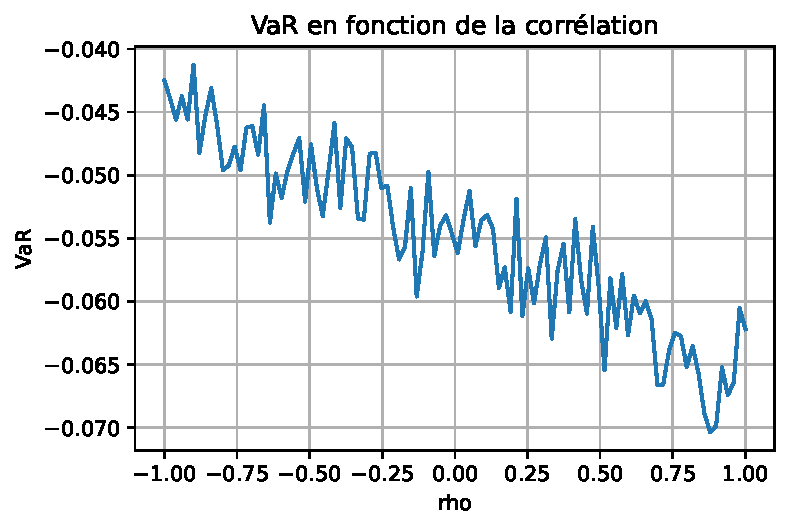
\includegraphics[keepaspectratio]{TP-3_files/figure-pdf/cell-26-output-2.pdf}}

\paragraph{Estimation de la volatilité du spread de
crédit}\label{estimation-de-la-volatilituxe9-du-spread-de-cruxe9dit}

Pour la volatilité du spread, nous avons supposé que
\(\sigma_s = 40\%\). Nous allons maintenant estimer cette volatilité à
partir des données de marché, en utilisant l'historique des spreads de
crédit sur une période de 5 ans, i.e.~11/03/2025 - 11/03/2020,
disponible sur ce \href{cds.xlsx}{lien}.

La volatilité du spread est une volatilité annualisée. De ce fait, la
formulation de la volatilité empirique, lorsque la fréquence est
quotidienne, est la suivante :

\[
\sigma_s = \sqrt{\frac{1}{n-1} \sum_{i=1}^{n} (s_i - \bar{s})^2} \times \sqrt{255}
\]

\begin{Shaded}
\begin{Highlighting}[]
\NormalTok{cds\_df }\OperatorTok{=}\NormalTok{ pd.read\_excel(}\StringTok{"cds.xlsx"}\NormalTok{, skiprows}\OperatorTok{=}\DecValTok{6}\NormalTok{)}
\CommentTok{\#date as date}
\NormalTok{cds\_df[}\StringTok{"Date"}\NormalTok{] }\OperatorTok{=}\NormalTok{ pd.to\_datetime(cds\_df[}\StringTok{"Date"}\NormalTok{], }\BuiltInTok{format}\OperatorTok{=}\StringTok{"\%Y{-}\%m{-}}\SpecialCharTok{\%d}\StringTok{"}\NormalTok{)}
\NormalTok{cds\_df }\OperatorTok{=}\NormalTok{ cds\_df.set\_index(}\StringTok{"Date"}\NormalTok{)}
\NormalTok{cds\_df }\OperatorTok{=}\NormalTok{ cds\_df.sort\_index()}

\NormalTok{cds\_df.head()}
\end{Highlighting}
\end{Shaded}

\begin{longtable}[]{@{}ll@{}}
\toprule\noalign{}
& PX\_LAST \\
Date & \\
\midrule\noalign{}
\endhead
\bottomrule\noalign{}
\endlastfoot
2020-03-11 & 30.772 \\
2020-03-12 & 36.977 \\
2020-03-13 & 37.869 \\
2020-03-16 & 44.432 \\
2020-03-17 & 49.923 \\
\end{longtable}

\begin{Shaded}
\begin{Highlighting}[]
\NormalTok{vol\_est }\OperatorTok{=}\NormalTok{ np.std(cds\_df[}\StringTok{"PX\_LAST"}\NormalTok{].pct\_change())}
\BuiltInTok{print}\NormalTok{(}\SpecialStringTok{f"Volatilité estimée sur 5 ans: }\SpecialCharTok{\{}\NormalTok{vol\_est}\OperatorTok{*}\NormalTok{np}\SpecialCharTok{.}\NormalTok{sqrt(}\DecValTok{255}\NormalTok{)}\SpecialCharTok{:.4f\}}\SpecialStringTok{"}\NormalTok{)}

\CommentTok{\# volatilité sur 1 an}
\NormalTok{vol\_est}\OperatorTok{=}\NormalTok{ np.std(cds\_df.loc[}\StringTok{"2024{-}03{-}11"}\NormalTok{:}\StringTok{"2025{-}03{-}11"}\NormalTok{, }\StringTok{"PX\_LAST"}\NormalTok{].pct\_change())}
\BuiltInTok{print}\NormalTok{(}\SpecialStringTok{f"Volatilité estimée sur 1 an : }\SpecialCharTok{\{}\NormalTok{vol\_est}\OperatorTok{*}\NormalTok{np}\SpecialCharTok{.}\NormalTok{sqrt(}\DecValTok{255}\NormalTok{)}\SpecialCharTok{:.4f\}}\SpecialStringTok{"}\NormalTok{)}
\end{Highlighting}
\end{Shaded}

\begin{verbatim}
Volatilité estimée sur 5 ans: 0.4512
Volatilité estimée sur 1 an : 0.5181
\end{verbatim}

\section{Asset management : autres types de
risques}\label{asset-management-autres-types-de-risques}

En dehors du risque de crédit et du risque de marché, il existe d'autres
types de risques qui peuvent affecter les institutions financières et
les marchés. Deux d'entre eux sont le risque de modèle et le risque
climatique.

\subsection{Risque de modèle}\label{risque-de-moduxe8le}

Le risque de modèle est le risque associé à une mauvaise utilisation
d'un modèle dans le processus de prise de décision. Il peut être causé
par :

\begin{itemize}
\tightlist
\item
  une incertitude sur les paramètres,
\item
  une qualité insuffisante des données,
\item
  ou une inadéquation structurelle du modèle par rapport à la réalité
  observée.
\end{itemize}

Ce risque peut conduire à des erreurs de prévision, à des décisions
inappropriées ou à des pertes financières. Il est donc essentiel de bien
comprendre les hypothèses et limites des modèles employés.

C'est une activité où l'intervention humaine reste indispensable : il
est nécessaire de procéder à des \emph{sanity checks}, du
\emph{backtesting}, et de challenger les modèles à l'aide de versions
plus simples (\emph{dégénérées}) ou plus riches, afin d'en comparer les
résultats et de mieux cerner leurs faiblesses.

Pour réduire le risque de modèle, il est courant de mettre en place une
fonction indépendante de validation, généralement assurée par les
équipes MRM (Model Risk Management). Ces dernières sont chargées :

\begin{itemize}
\tightlist
\item
  d'auditer les modèles,
\item
  de mener des tests de robustesse,
\item
  et de recommander des provisions en cas de risque de surévaluation des
  actifs.
\end{itemize}

Les compétences clés pour cette activité incluent : - les mathématiques
financières, - la connaissance des marchés financiers et des modèles de
risque, - la programmation et l'utilisation d'outils quantitatifs, -
ainsi que des aptitudes à la communication, au travail en équipe et au
raisonnement critique.

\subsection{Risque climatique}\label{risque-climatique}

Le risque climatique désigne les impacts potentiels des changements
climatiques et des politiques environnementales sur les entreprises et
les marchés financiers. Contrairement aux risques classiques, les
trajectoires de référence sont définies par des organismes scientifiques
comme le GIEC, ce qui limite l'appropriation directe des modèles par les
institutions financières. Il s'agit donc d'un domaine où le risque de
modèle est indirect.

Le réseau NGFS (Network for Greening the Financial System) a été mis en
place pour aider les régulateurs et les banques centrales à mieux
intégrer les risques climatiques dans leurs cadres prudentiels.

À l'heure actuelle, il n'existe pas de consensus clair sur la manière
d'intégrer pleinement le risque climatique dans les modèles financiers ;
il s'agit plutôt de tentatives progressives d'adaptation. Le NGFS
propose plusieurs scénarios climatiques, parmi lesquels :

\begin{itemize}
\tightlist
\item
  Current Policies : continuité des politiques actuelles sans nouvel
  engagement.
\item
  NDC (Nationally Determined Contributions) : politiques actuelles +
  engagements annoncés par les États.
\item
  Disorderly Transition (1.5°C) : les engagements sont mis en œuvre avec
  retard ou de façon désorganisée.
\item
  Net Zero / 2°C : scénario optimisé pour limiter le réchauffement à 2°C
  --- le cadre le plus ambitieux et le plus stable.
\end{itemize}

On distingue généralement deux types de risques climatiques :

\subsubsection{1. Risque physique}\label{risque-physique}

Ce risque est lié aux conséquences directes des changements climatiques
sur les infrastructures et l'environnement : - Risques aigus :
événements extrêmes (inondations, sécheresses, tempêtes, etc.). -
Risques chroniques : évolutions lentes (élévation du niveau des mers,
hausse des températures, etc.).

Ces risques peuvent entraîner : - des pertes matérielles, - des
interruptions d'activité, - des coûts de réparation et d'adaptation.

\subsubsection{2. Risque de transition}\label{risque-de-transition}

Ce risque est associé aux mesures prises pour réduire les émissions de
gaz à effet de serre et passer à une économie bas carbone. Il peut
provoquer : - des pertes de valeur sur certains actifs, - des coûts de
transition élevés, - des bouleversements sectoriels et technologiques.

Il comprend deux composantes : - le risque politique (durcissement
réglementaire, interdictions, fiscalité verte, etc.), - et le
risque/opportunité technologique (émergence de nouvelles technologies,
changement dans les préférences de consommation, etc.).

On peut formuler ce risque comme une relation :

\[
\text{Risque de transition} = \text{Risque politique} - \text{Opportunités technologiques}
\]

Ainsi, une entreprise bien positionnée sur les technologies vertes peut
compenser tout ou partie du risque politique subi.

\begin{itemize}
\tightlist
\item
  Le risque physique est plus élevé dans les scénarios Current Policies,
  NDC, et Disorderly Transition, car ils impliquent une action
  climatique insuffisante ou retardée.
\item
  À l'inverse, le risque de transition est plus important dans les
  scénarios ambitieux comme Net Zero, où les ajustements politiques et
  économiques sont rapides et profonds.
\end{itemize}




\end{document}
